\chapter{实验分析与讨论}
本章将详细描述本文所使用的数据集,实验设计以及对于实验结果的评价标准。本文在第三章提出了
在网络表征算法HLE及其增量表征算法iHLE,第四章中提出了在属性网络中的表征算法SR及其增量网络场景下的表征算法iSR,本章将在数据集上进行相关的实验并与其他著名算法进行对比分析。

%%%%%%%%%%%%%%%%%%%%%%%%%%%%%%%%%%%%%%%
%----------------------------------------     数据介绍     ---------------------------------------%
%%%%%%%%%%%%%%%%%%%%%%%%%%%%%%%%%%%%%%%
\section{数据介绍}
本文利用的数据集为4个真实数据集,其中真实数据集包括2个社交媒体数据和2个引用网络数据,这些数据集曾在\cite{li2017attributed,tang2015line}中使用,且都是在线公开数据\footnote{https://linqs.soe.ucsc.edu/data}\footnote{people.tamu.edu/~xhuang/Code.html}。
\begin{itemize}
	\item \textbf{BlogCatalog}: BlogCatalog是一个社交媒体网站,用户在上面发表博客并通过相互关注建立网络,数据集选取了5196个用户节点,包含了171,743条连边。用户节点的属性信息来自用户博客的关键词描述加工处理而成,构建了8189维用户节点的属性特征,用户的分类标签是从用户自定义的兴趣爱好中选择得来的。
	
	\item \textbf{Flickr}:Flickr是一个图片分享社区,用户通过图片分享与其他用户交互,数据集以用户间的相互关注组成网络,数据集选取了7575个用户节点,包含了239,728条连边,用户节点的属性信息来源于用户的分享内容的标签(tag)信息,提取了12047维节点属性特征。用户的类别信息来源于用户加入的兴趣社区。
	
	%\item \textbf{Citeseer}:Citeseer数据集是从挑选Citeseer网站上的一些文献,文献的选择过程保证对于每一篇文献都有至少被一篇文献所引用,总共选取了3312篇文章作为网络中的节点,构建了一个文献引用网络。文献的属性是来自对内容的处理得到,通过去掉停用词和选取词干的方法,剩下的3703个单词组成词库,在对文献进行处理的时候,出现次数小于10的单词去掉,根据文献中是否存在词库对应单词,将对应特征置为0/1,于是文献节点属性特征维数为3703维。根据文献本身所属主题,文献被分为六个类别:Agents,AI,DB,IR,ML和HCI。
	
	%\item \textbf{Cora}:Cora是另一个论文引用网络,主要是机器学习细分领域的论文之间的引用关系,同样在构造数据集的时候保证最后每一篇论文都有至少有一个被引用量,该数据集包含2708篇论文,在提取论文节点的属性特征时,采用方法跟Citeseer类似,通过对全部文献去掉停用词、处理词干构建词库,去掉每篇文章中的出现少10次的词,得到1433维属性特征。根据论文的内容,将论文节点分成6种:Case Based, Genetic Algorithms, Neural和Networks, Probabilistic Methods, Reinforcement Learning, Rule learning和 Theory。
	
	\item \textbf{PubMed}: PubMed是另一个论文引用网络,主要涉及的是生物领域的文献。数据集选取了19717个论文作为网络节点,不同的是,论文节点的属性特征不是0/1型,而是用文档中对应单词TF-IDF加权得到。数据集中论文根据研究主题被分成3类:Diabetes Mellitus Experimental,Diabetes Mellitus Type 1和Diabetes Mellitus Type 2。
	
	\item \textbf{DBLP}:DBLP数据集是从挑选DBLP网站上的一些文献,文献的选择过程保证对于每一篇文献都有至少被一篇文献所引用,总共选取了781,109篇文章作为网络中的节点,构建了一个文献引用网络。文献的属性是来自对内容的处理得到,通过去掉停用词和选取词干的方法,剩下的5703个单词组成词库,在对文献进行处理的时候,出现次数小于10的单词去掉,根据文献中是否存在词库对应单词,将对应特征置为0/1。根据文献本身所属会议,文献被分为7个类别:AAAI,CIKM,ICML,KDD,NIPS, SIGIR和WWW。
	
\end{itemize}
关于上述数据的具体详情,见下表,另给出BlogCatalog数据集中的度分布情况。
\begin{table}
\centering
\caption{使用数据集详细统计信息}
\begin{tabular}{C{1in}C{1in}C{1in}C{1in}C{1in}}
\textbf{数据集} & \textbf{节点数} &\textbf{连边数} & \textbf{属性数}&\textbf{类别数}\\ \hline 
BlogCatalog & 5186  & 171,743 &8189&6\\
Flickr	& 7575 &239,728 & 12,047 & 9 \\
%Citeseer& 3312 & 4536  &  3703 & 6 \\
%Cora & 2708 &5429 & 1433 &7 \\
PubMed & 19,717 &44,338&500 &3 \\
DBLP & 781,109 &4,191,677&5703 & 7 \\
\hline

\end{tabular}
\end{table}

%\begin{figure}
%	\centering
%	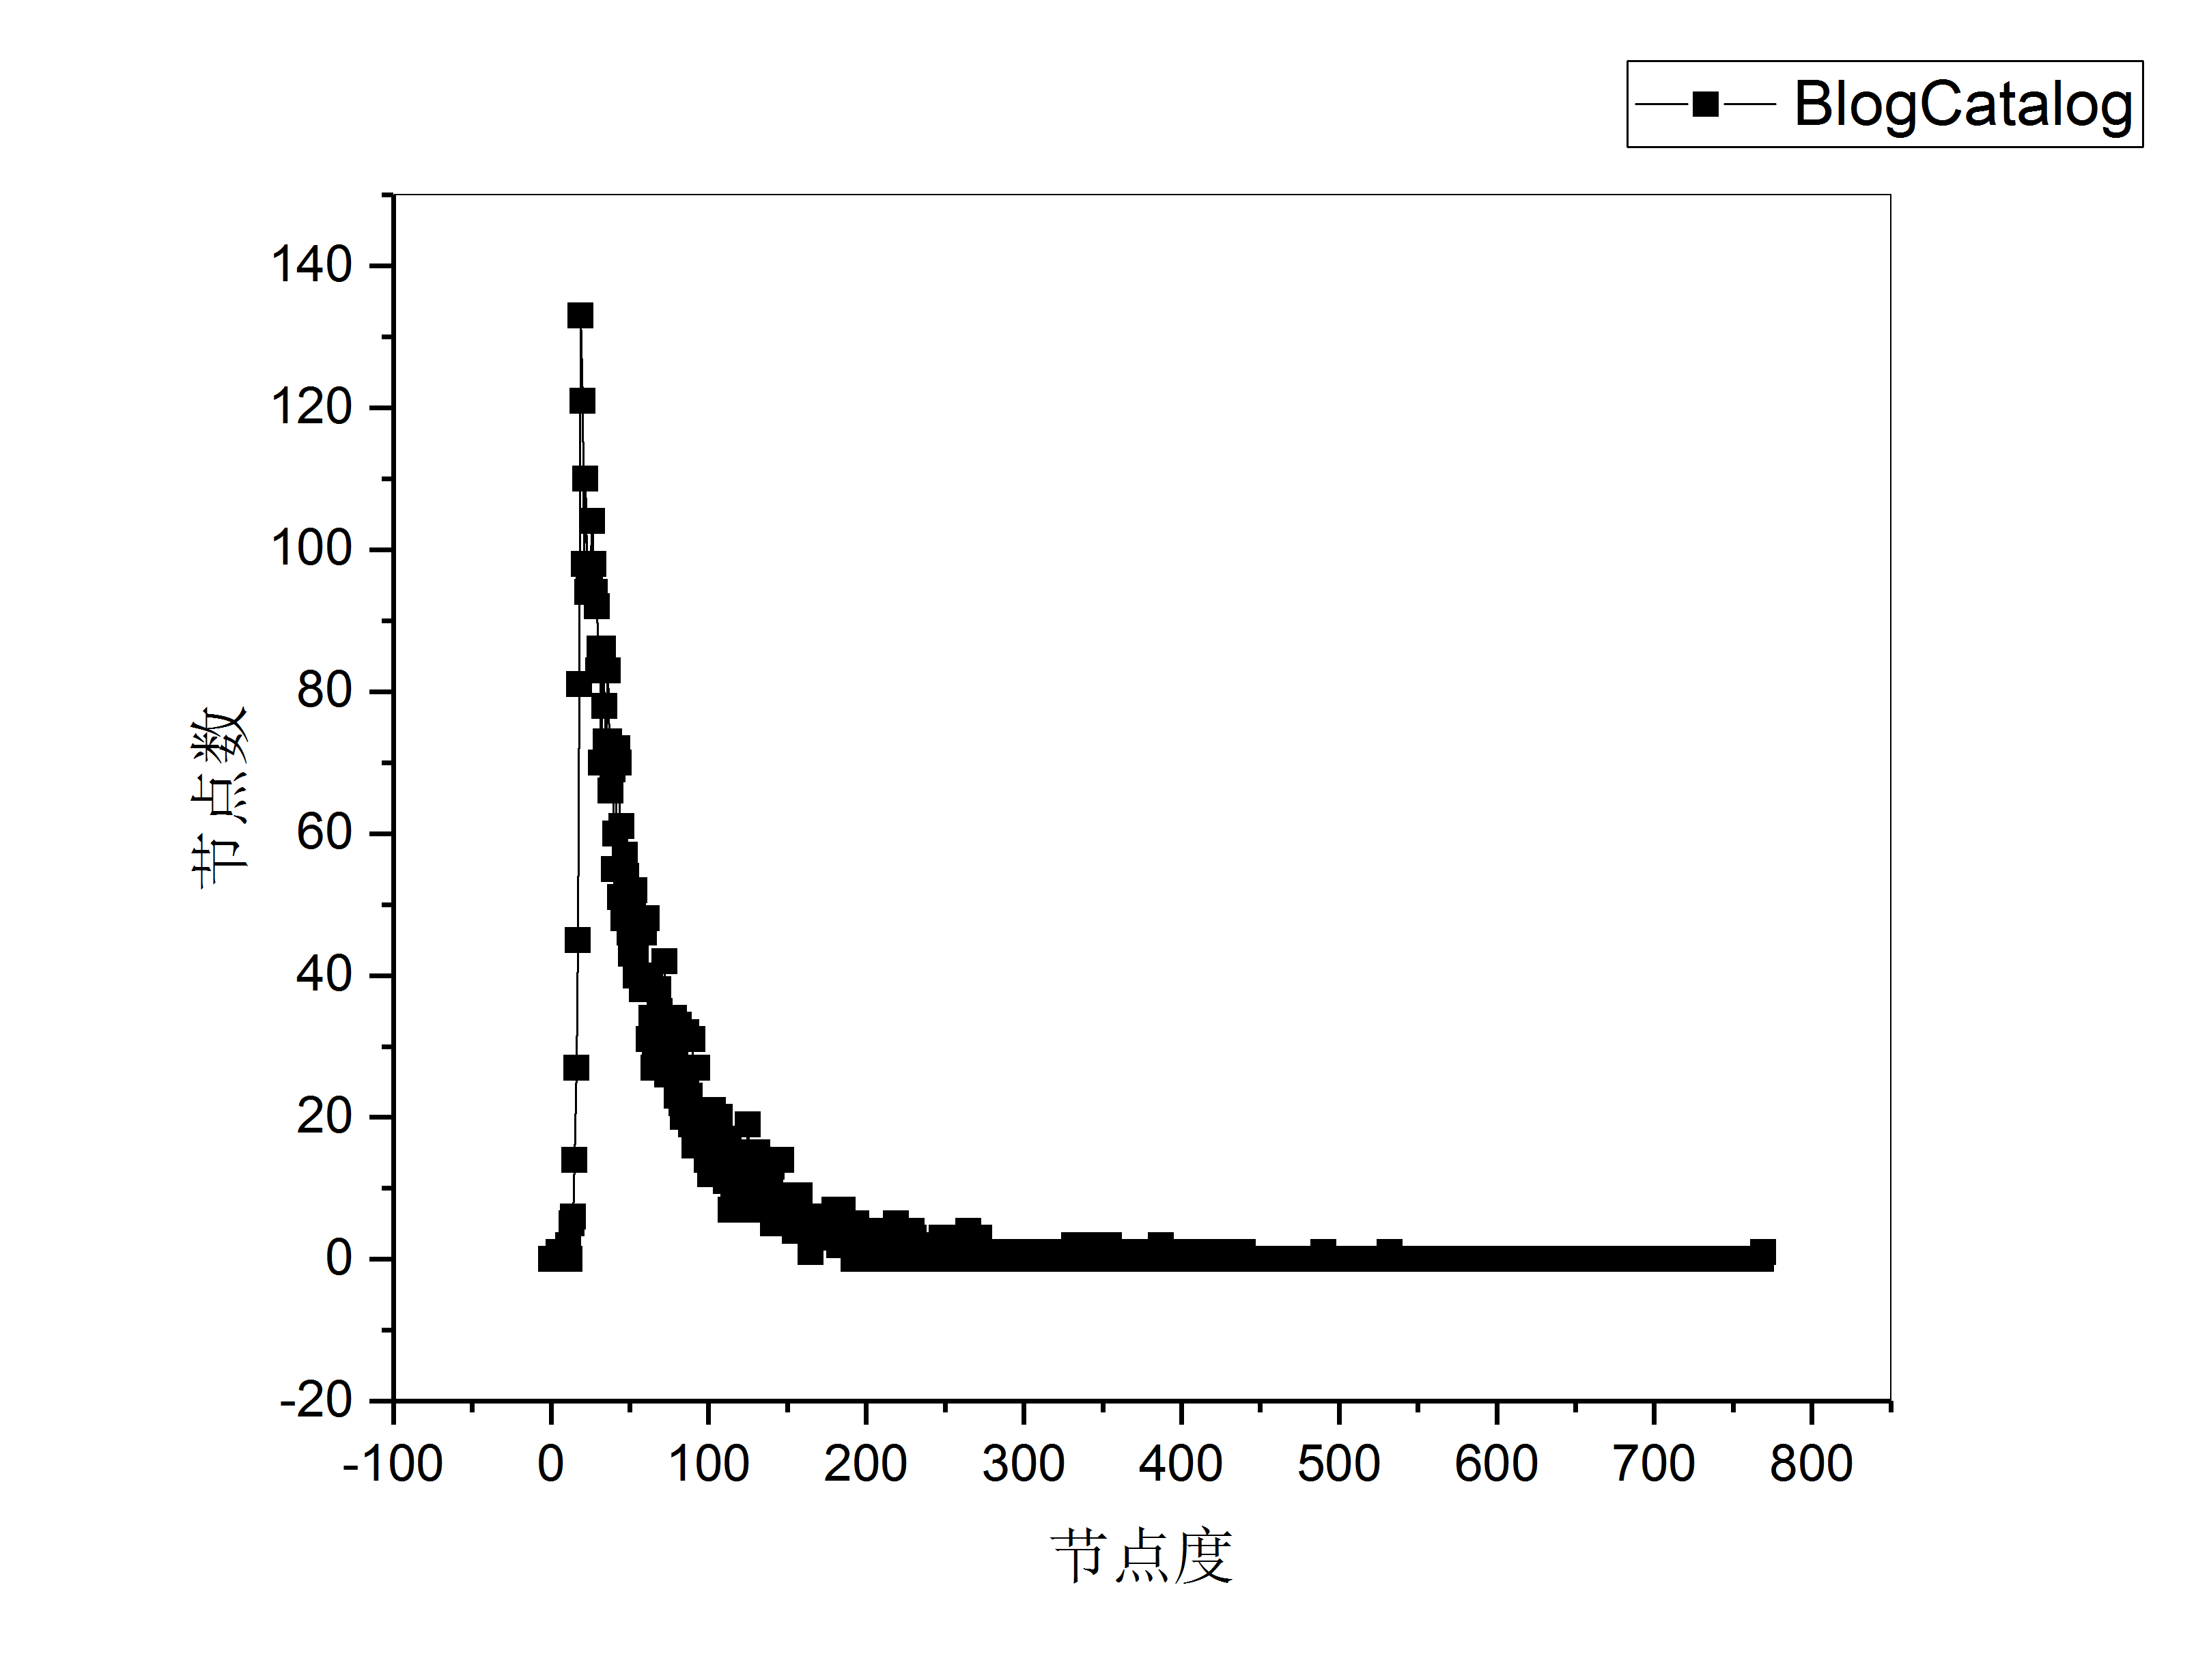
\includegraphics[width=5in]{figures/blogCatalog_degree}
%	\caption{案例数据:BlogCatalog中的度分布}
%\end{figure}
\section{实验环境}
实验的硬件环境与软件环境如表\ref{my-label5_1}所示:

\begin{table}[]
	\centering
	\caption{实验硬件与软件环境表}
	\label{my-label5_1}
	\begin{tabular}{@{}llll@{}}
		\toprule
		硬件配置\\ \midrule
		处理器&	Intel@CoreTM i7-5820k CPU @3.3GHz x 12\\ \midrule
		内存&	128G\\ \midrule
		硬盘&	1T\\ \midrule
		软件配置 \\ \midrule
		操作系统&	Ubuntu 16.04 LTS \\ \midrule
		开发环境&	Python 2.7  \\ \bottomrule
	\end{tabular}
\end{table}

\section{实验设计}
图表征算法是对网络中节点进行向量表征的过程,在这一部分主要从两方面对前面章节提出的算法进行分析评价:
\begin{itemize}
	\item \textbf{准确性}:图表征算法学习到的向量表征需要应用于后续的机器学习任务,在不同的机器学习任务中表现出来的分类预测效果如何,跟其他算法对比效果上的差异。
	\item \textbf{运行效率}:基于动态增量场景提出的算法运行效率如何,跟其他离线批量算法在效率上的差异。
\end{itemize}
本节将分别从这两方面提出设计的实验过程。
\subsection{准确性评估}
在准确性评估这一部分,本章主要针对两个学习任务来进行具体的对比:一个是节点多分类任务,一个是图挖掘中常见的链路预测问题。对于不同的学习任务有不同的实验设计过程和评价准则,下面将分别对这些实验的具体过程进行介绍。

\subsubsection{节点多分类实验}
\textbf{节点多分类实验}:节点多分类问题是一个监督学习任务,在对节点进行向量表征之后需要划分训练集和测试集,通过训练集训练模型,对测试集中的数据进行预测并评估结果的好坏。分类问题的评估方法有很多,不同于普通的二分类问题,节点分类问题是多分类过程,在节点分类任务中一般采用的评测指标有三种:分类准确率(accuracy), F1-Macro和F1-Micro,实验中将用到不同的评测指标。



{\textbf{衡量指标1:F1-Macro和F1-Micro}}在介绍这两个评价准则之前,需要介绍F1值。在二分类问题中,根据实际的类别标签和预测的类别标签的不同情况可以得到混淆矩阵:
\begin{table}
	\centering
	\caption{混淆矩阵}
	\begin{tabular}{|c|c|c|c|}
		\hline
		\multirow{2}*{预测标签}& \multicolumn{2}{|c|}{真实标签} \\
		\cline{2-3}
		~ & 正例 & 反例 \\ \hline
		正例 & TP(真正例) & FP(假正例) \\ \hline
		反例 & FN(假反例) & TN(真反例) \\
		\hline
	\end{tabular}
\end{table}

其中精度P(Precision)和召回率R(Recall)可以根据混淆矩阵定义出来:
\begin{equation}
\begin{aligned}
P &= \frac{\#TP}{\#TP+\#FP} \\
R &= \frac{\#TP}{\#TP+\#FN}
\end{aligned}
\end{equation}
其中$\#\cdot$表示对应样本的个数,考虑在现实场景中精度和召回率各有不足,召回率偏向于将样本都预测为正样本,精度需要保证预测中真实正样本的比例,会偏向于将预测正样本的个数降低,F1值综合考虑精度和召回率,对两者进行统一:
\begin{equation}
	F1 = \frac{2\times P\times R}{P+R}
\end{equation}
可以看出$F1$为精度和召回率的调和平均。

在多分类问题中,无法通过二元的混淆矩阵来表示样本预测与真实之间的关系,对于$F1$因此有了在多分类情况的变形F1-macro和F1-micro。在多分类场景下需要将不同类别两两之间计算混淆矩阵,算出对应的精度和召回率,F1-macro的计算方法是:
\begin{equation}
	macro\-P = \frac{1}{n}\sum P_i
\end{equation}
\begin{equation}
macroR = \frac{1}{n}\sum R_i
\end{equation}
\begin{equation}
F1macro = \frac{2\times macroP\times macroR}{macroP+macroR}
\end{equation}
在计算完混淆矩阵后,对所有矩阵的对应值去平均得到$\overline{TP}, \overline{TN}, \overline{FN},\overline{FP}$,可以得到F1-micro的计算方法:
\begin{equation}
microP = \frac{\overline{TP}}{\overline{TP}+\overline{FP}}
\end{equation}
\begin{equation}
microR = \frac{\overline{TP}}{\overline{TP}+\overline{FN}}
\end{equation}
\begin{equation}
F1micro = \frac{2\times microP\times microR}{microP+microR}
\end{equation}

对于节点多分类问题,本章对所有数据集进行比例抽样,90\%作为数据训练集,10\%作为测试集,多分类学习任务采用逻辑斯蒂回归LR(Logistic Regression)算法进行学习,并通过F1-macro,F1-micro两个指标对算法效果进行评估。在对算法进行准确性评判时,对比实验过程分成两个部分:\textbf{离线模型}和\textbf{增量模型}。对于\textbf{离线模型}跟已有的图表征算法的效果进行对比:
\begin{itemize}
	\item 拉普拉斯特征映射算法LE:基于保留一阶接近度的图表征方法,将问题转化为求矩阵特征值的问题
	%\item 图分解算法GF(Graph Factorization):基于保留一阶接近度的图表征方法,采用梯度下降方式优化求解表征向量。
	\item LINE算法:通过保留一阶接近度和二阶接近度进行图表征的算法,通过负采样优化计算。
	\item Node2Vec算法:借用自然语言处理中的Word2vec思想,通过随机游走生成节点语料库,从而对图进行表征学习。
	\item CCA算法\cite{hardoon2004canonical}:将原始网络结构和原始属性特征融合进行降维作为节点分类任务的输入。
	\item TADW算法\cite{yang2015network}%\footnote{https://github.com/xhuang31/AANE\_python}
	:将网络结构特征和属性特征同时进行优化,得到属性网络表征作为后续学习任务的输入。
	\item HLE算法:本文提出的基于高阶接近度的拉普拉斯特征映射算法。
	\item SR1算法:本文提出的基于属性相似度的表征算法。
	\item SR算法:本文提出的SR1优化算法。
\end{itemize}
通过下面的表对实验中采用的算法进行分类:
\begin{table}
	\centering
	\caption{节点分类任务图表征算法分类}
	\begin{tabular}{|C{2in}|C{3in}|}
		\hline
		\textbf{类别} & \textbf{算法} \\ \hline 
		\multirow{4}*{网络表征}&拉普拉斯特征映射算法LE \\ 
		\cline{2-2}
		%~ &	 图表征算法GF \\ \cline{2-2}
		~ &  LINE算法	\\ 	\cline{2-2}
		~ &	 Node2Vec算法 \\ \cline{2-2}
		~ &  HLE算法	\\ \hline
		属性表征 & SR1算法 \\ \hline
		\multirow{4}*{属性网络表征} & CCA算法 \\ \cline{2-2}
		~ & TADW算法 \\ \cline{2-2}
		~ & SR算法 \\ \cline{2-2}
		~ & HLE+SR算法 \\ \hline
	\end{tabular}
\end{table}

\textbf{增量模型}的准确性评估实验不同于离线模型的实验设计。在离线模型评估中采用的方式为随机按比例抽样进行学习任务,不同比例的样本不存在包含关系。而在线模型中将样本分成不同的时间步,依次加入网络中进行,因此后一个时间步包含前一个时间步的样本整体。在这里需要注意的一点是,在实验过程中抽样过程先于表征算法,先完成抽样再进行表征学习,在节点分类任务时存在的训练测试集分割则在表征算法之后进行。对于在线模型,实验过程主要跟对应的离线模型进行准确性对比。

在对图表征算法进行准确性评判,本文还将表征向量应用于链路预测实验。
\subsubsection{链路预测实验}
\textbf{链路预测实验}:链路预测问题也是一个监督学习任务,但是不同于节点多分类任务的标签来源于其他附加信息,链路预测问题的标签来源于网络中的连边。链路预测问题的初衷是根据网络结构中已经存在的连边,预测没有产生连接的节点对中产生连接的概率,链路预测问题原本是基于网络对网络的学习,进一步扩展在属性网络中,利用节点本身的属性特征提高预测效果。

\textbf{属性网络中的链路预测}:给定无向属性网络$G(V,E,H)$,其中$V$代表节点集合,$E$代表连边的集合,$H$代表网络节点的属性特征集合,根据节点集合可以算出网络中所有可能连边的集合为$U$,集合的大小为$|U| = \frac{|V|(|V|-1)}{2}$,链路预测问题就是需要通过一定的算法对连边$E\prime\in U\setminus E$的可能性进行预测,也即对不存在(或未被观测到)的连边预测存在的概率。

在传统的监督学习任务中每条样本对应有特征和一个(或多个)类别标签,在模型训练之前划分训练集和测试集。本文中的链路预测也需要进行训练集和测试集的划分,在训练集中需要包含正样本和负样本,测试集也同样需要包含正负样本,正样本为在网络中确实存在的连边,也即$E$中连边,负样本连边来源于$U\setminus E$,关于训练集和测试集的划分过程如下图:
\begin{figure}
	\centering
	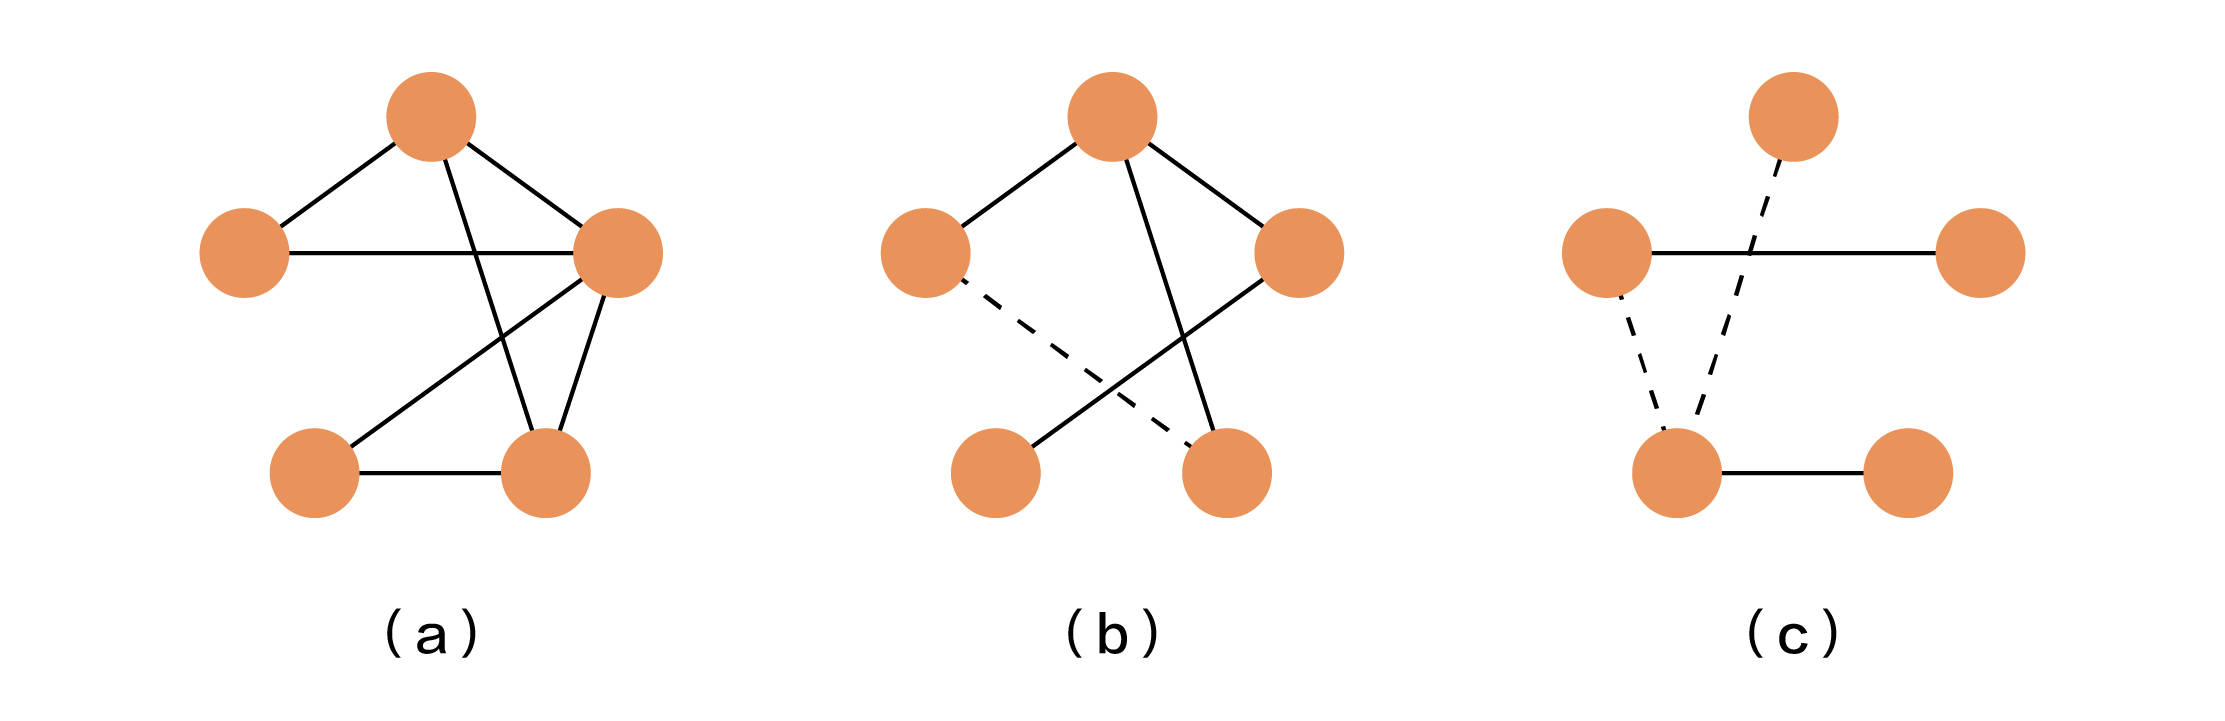
\includegraphics[width=5in]{figures/link_prediction_split}
	\caption{链路预测训练测试集划分:(a)全部连边$E$;\\(b)训练集:包含正负样本,负样本用虚线表示(c)测试集:包含正负样本}
\end{figure}

不同于上面的节点分类任务,在链路预测实验中不是直接针对节点进行k折交叉验证实验,链路预测的训练测试集是针对连边进行采样得到的,图表征算法学习到的是节点的向量表征,将图表征用于链路预测任务的直观方法是,将关于连边$e$的节点对$(i,j)$的表征向量$X_i,X_j$的函数$f(X_i, X_j)$作为该连边$e$的特征,在本文实验中采用$f(X_i, X_j) = X_i\circ X_j$ ,也即$X_i, X_j$对应元素相乘作为边的特征,再放入二分类的学习算法中,在实验中本文采用的分类算法是逻辑斯蒂回归(Logistic Regression),实验效果在测试集上进行通过\textbf{AUC}和\textbf{准确率}进行效果评价,下面分别介绍一下两种评价标准。

{\textbf{衡量指标1:分类准确率ACC}} :准确率的定义是对于给定的测试样本集,分类模型预测类别正确的样本占总样本的比例,从损失函数的角度来讲,就是模型损失函数为0-1阶梯函数时测试集上的损失值。

\textbf{衡量指标2:AUC}:AUC(Area under ROC curve),意思就是ROC(Receiver Operating Characteristic)曲线下的面积,ROC曲线是以FPR为横轴,TPR为纵轴的坐标中画出的曲线,关于FPR和TPR可以根据混淆矩阵定义:
\begin{equation}
	TPR = \frac{\#TP}{\#TP+\#FN}
\end{equation}
\begin{equation}
FPR = \frac{\#FP}{\#TN+\#FP}
\end{equation}
ROC曲线将样本按照预测概率从大到小排序,从第一个样本依次设置分类阈值为其预测值,并以此对所有样本判定预测的正负值,进一步计算出一组TPR和FPR值,以此循环可以得到一系列的值形成ROC曲线,AUC表示ROC曲线与横轴FRP围成的面积大小,AUC评价方法关注的是预测样本概率的排序质量。

 同样的,在这一部分增量学习算法主要跟对应的离线算法进行准确性对比,链路预测的实验过程图\ref{fig:link_prediction_process}所示:
\begin{figure}
	\centering
	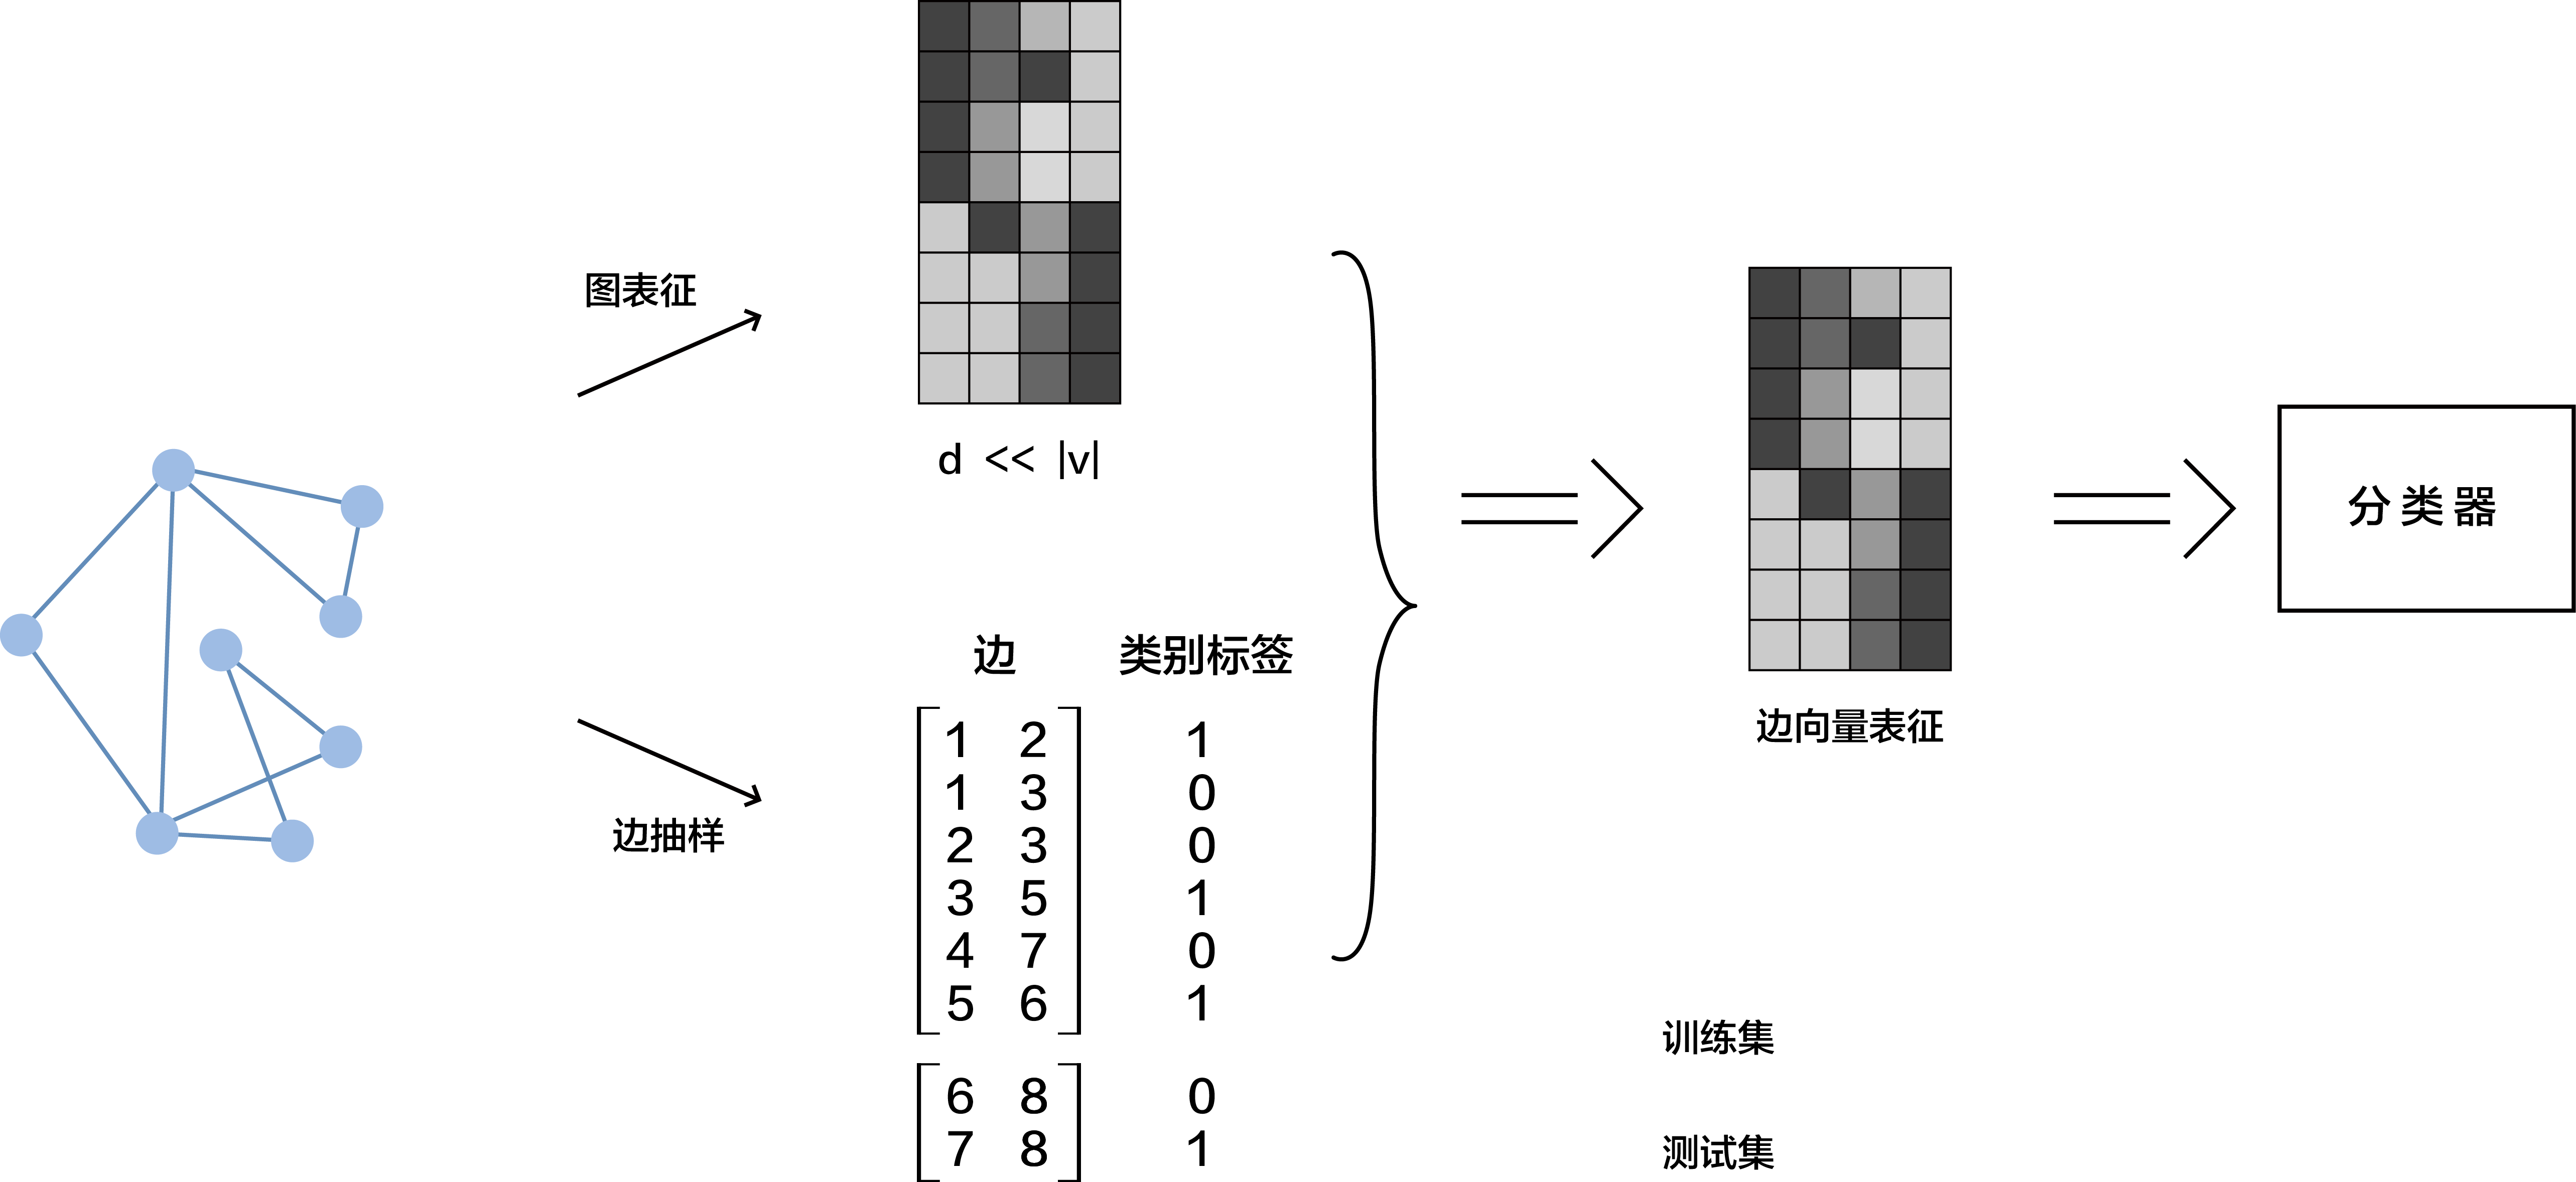
\includegraphics[width=6in]{figures/link_predict_frame}
	\caption{链路预测实验过程}
	\label{fig:link_prediction_process}
\end{figure}

\subsection{运行效率评估}
在运行效率评估这一部分,主要进行增量算法跟离线算法之间的对比,将数据集分解成多个时间步,在最初的时间步采用离线算法进行图表征,在第二个及以后时间步将分成增量算法和离线算法进行表征学习,并从两方面来对算法效果进行对比评估。
\begin{itemize}
	\item \textbf{累积运行时间}。将全部数据集分成不同时间步,计录并比较从第一个时间步到最后一个时间步之间累积所用的运行时间。
	\item \textbf{不同表征维度的效率对比}。对比在不同表征维度时,增量算法运行所有时间步所累积时间相对于离线模型的速度提升。 
\end{itemize}
\subsection{实验数据处理过程}
\textbf{关于链路预测的抽样过程}:
在链路预测进行边采样时,为保证训练集中包含所有节点,随机采样的方式需要不断验证网络的连通性和节点数,复杂度较高,在本文中采用基于最小生成树的方式抽取网络中最小生成树,训练集由最小生成树包含边集合与随机边集合组合而成。

 \textbf{关于增量实验的抽样过程}:已有的数据集是一个静态的网络数据,并不包含演化过程,因此需要通过节点抽样生成一个网络演化的过程,主要思想就是通过从原有网络中逐个去掉网络中的节点,记录下过程中删除的网络节点,在增量过程中则依次加入这些节点进行表征学习,过程如图\ref{fig:network_sample}中所示:
\begin{figure}
	\centering
	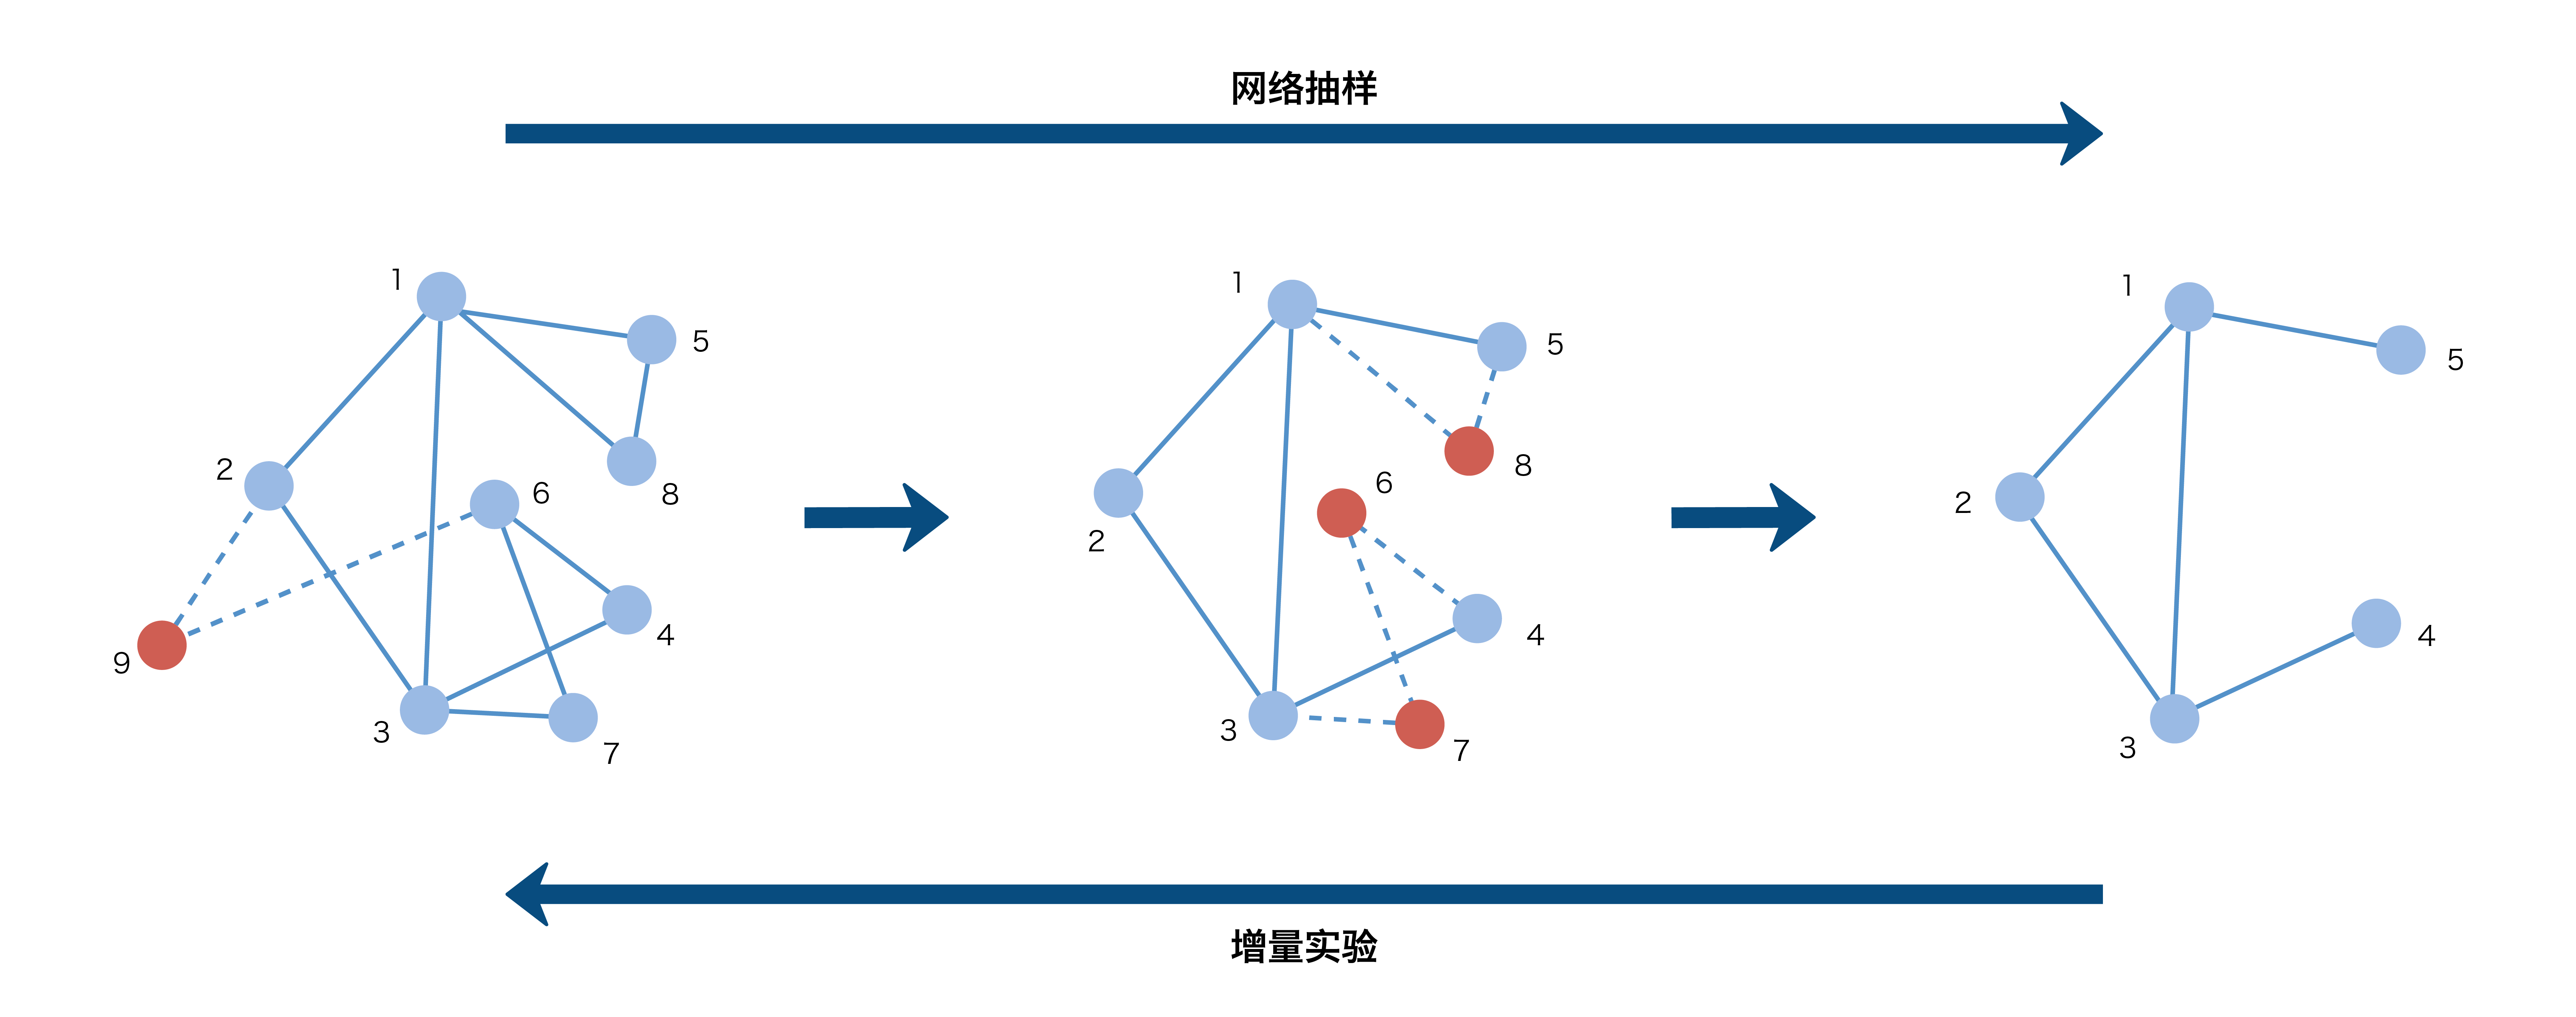
\includegraphics[width=6in]{figures/inc_sample}
	\caption{网络采样过程}
	\label{fig:network_sample}
\end{figure}


本文研究范围内,在网络不断地增量变化过程中,为保证节点在增量场景下进行有效表征,后加入的节点会跟先加入的节点进行连接,所以增量网络在每个时刻需要为全联通图,反之,在抽样过程中,抽样方法需要保证删除节点前后,子图个数不会增加。在这个基本要求下,随机选取节点进行删除会存在问题,会出现删除一个节点后网络变成非全联通的,于是在本章实验中考虑从节点重要性入手,以重要性逆序进行删除,衡量节点重要性的指标中比较简单的有节点度和PageRank值\cite{page1999pagerank},本章采用对节点重要性采用PageRank算法进行评估。于是在实验中采用基于Pagerank值大小逆序删除的方法进行网络抽样。
\begin{figure}
	\centering
	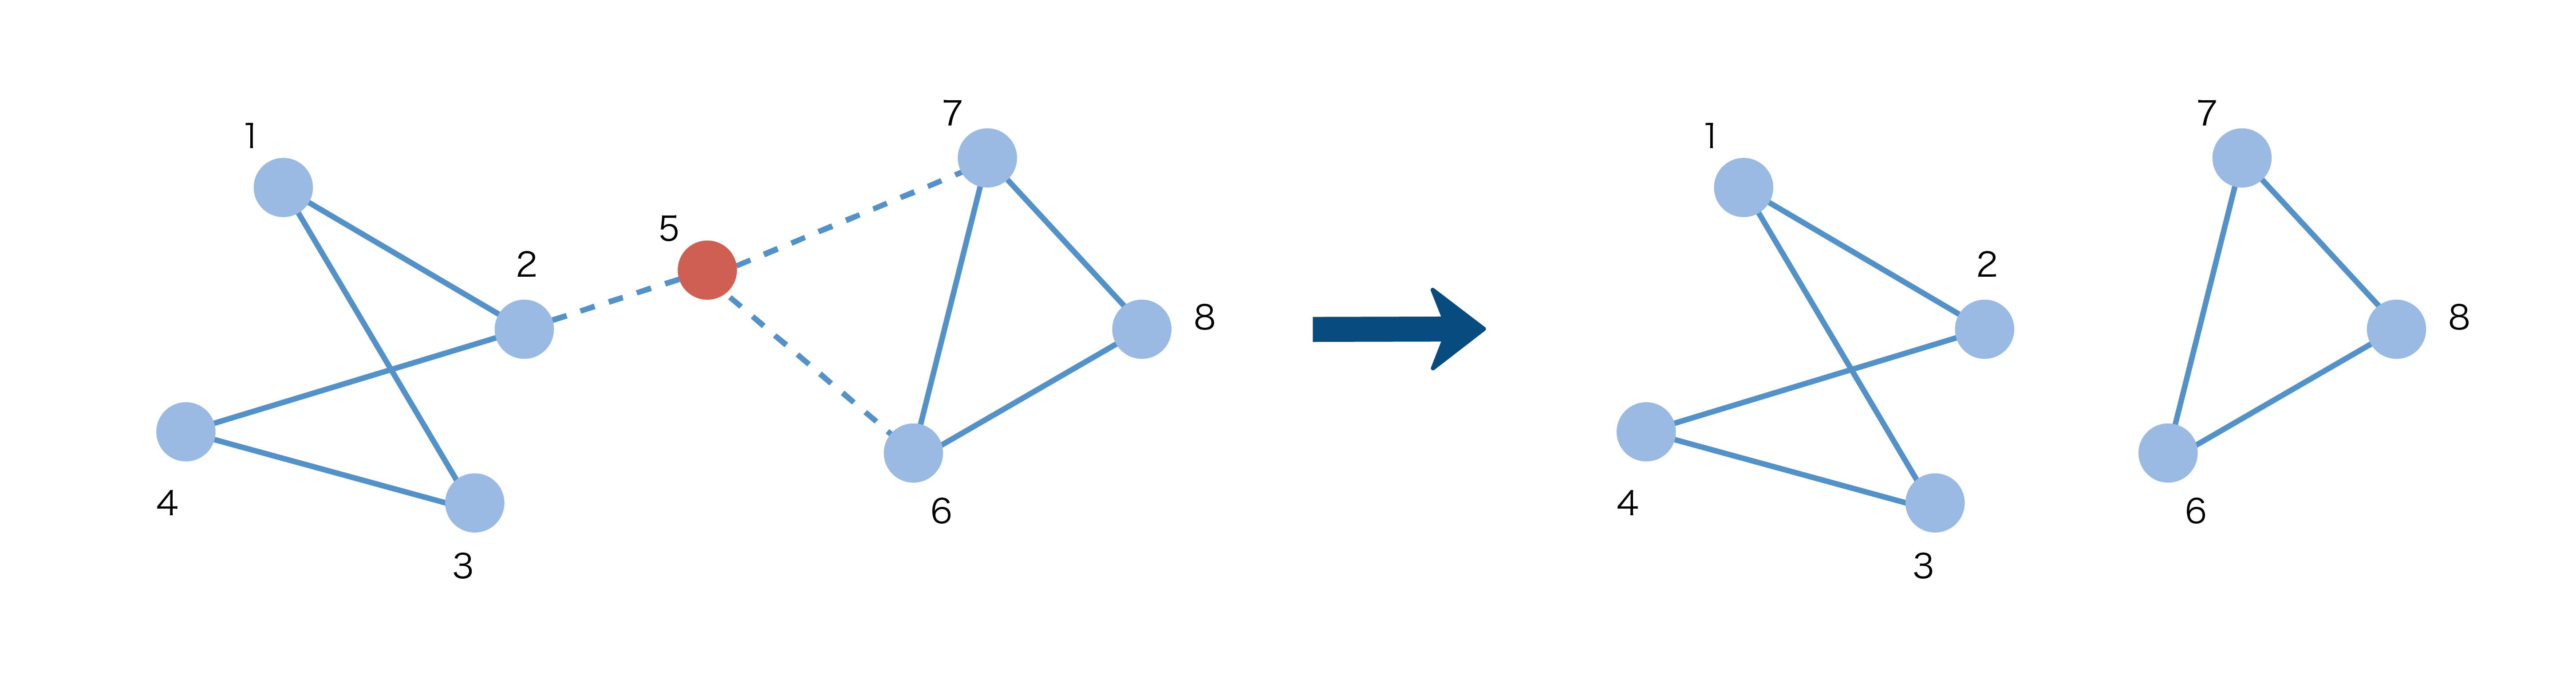
\includegraphics[width=6.2in]{figures/sample_split}
	\caption{随机采样可能出现问题}
\end{figure}


%%%%%%%%%%%%%%%%%%%%%%%%%%%%%%%%%%%%%%%
%----------------------------------------     实验结果与分析     ---------------------------------------%
%%%%%%%%%%%%%%%%%%%%%%%%%%%%%%%%%%%%%%%
\section{实验结果与分析}
\subsection{准确性评估}
在对表征算法进行准确性评估时任务主要分两方面:\textbf{离线模型}和\textbf{增量模型}。离线模型对比不同的算法,在图表征算法中表征向量的最佳维数为不确定的,在节点分类中,所有算法采用了(100,110,120,130,140,150)这6组表征维数,取最佳的表征结果记录,实验结果如表\ref{tab:static_node_classification}中所示,在同一数据集上的最佳结果用加黑标出。

其中\textbf{节点分类}实验中离线模型部分分成了三类:1.在只利用网络结构进行表征的算法中,HLE算法效果明显优于其他对比算法;2.在只利用节点属性信息进行表征学习的算法中,SR1算法的效果在BlogCatalog、DBLP和Flickr数据集上效果优于HLE算法,而在PubMed数据集上效果不如后者,可能的影响因素是在不同数据集中,节点属性所包含的特征信息跟网络结构所包含的特征信息量比重会不一致,前三个数据集节点属性信息量稍大一些,PubMed数据集节点属性则相反;3.在同时利用网络结构和节点属性的算法中,HLE+SR算法(HLE的表征向量并上SR算法的表征向量)结果明显优于其他算法。这其中SR算法的效果效果比CCA略优,但效果不够好,可能的原因是SR算法采用以结构为主导的属性相似度计算,网络结构上没有相连就没有属性相似度,在网络结构非常稀疏的情况下,会导致丢失大部分信息,在所有算法中纵向对比,结合网络信息和节点属性的算法普遍优于只有单方面信息的算法。

\begin{table}[]
	\centering
	\caption{离线模型在不同数据集上节点分类任务结果(单位为\%)}
	\label{tab:static_node_classification}
	\begin{tabular}{|c||c|c||c|c||c|c||c|c|}
		\hline
		数据集      & \multicolumn{2}{c||}{BlogCatalog} & \multicolumn{2}{c||}{Flickr}     & \multicolumn{2}{c||}{DBLP}   & \multicolumn{2}{c|}{PubMed}     \\ \hline\hline
		算法       & Micro        & Macro       & Micro       & Macro       & Micro       & Macro       & Micro       & Macro       \\ \hline
		LE       & 66.13           & 67.21          & 48.74          & 48.22          & 41.65          & 49.21          & 62.37          & 65.24          \\ \hline
		LINE     & 69.25           & \textbf{71.54} & 59.91          & 60.03          & 51.06          & 55.99          & 64.38          & 59.27          \\ \hline
		Node2Vec & 67.21           & 69.39          & 59.01          & 58.68          & \textbf{63.48}          & 60.95 & 80.61          & 79.30          \\ \hline
		HLE      & \textbf{69.31}  & 70.35          & \textbf{63.57} & \textbf{62.86} & 62.12 & \textbf{61.76}          & \textbf{81.26} & \textbf{80.28} \\ \hline\hline
		SR1      & 80.26           & 79.85          & 75.69          & 76.12          & 37.13          & 36.65          & 64.23          & 66.16          \\ \hline\hline
		CCA      & 48.53           & 47.69          & 26.02          & 27.31          & 35.24          & 36.42          & 51.12          & 52.11          \\ \hline
		TADW     & 84.95           & 84.99          & 85.51          & 84.63 & 65.32          & 62.09          & 88.58          & \textbf{88.41} \\ \hline
		SR       & 50.36           & 51.45          & 28.16          & 27.78          & 23.45          & 22.67          & 52.13          & 53.42          \\ \hline
		HLE+SR   & \textbf{85.12}  & \textbf{85.33} & \textbf{85.79} & \textbf{85.31}          & \textbf{66.12} & \textbf{63.15} & \textbf{88.76} & 87.16          \\ \hline
	\end{tabular}
\end{table}

准确性评估的另一个实验是链路预测,离线模型的链路预测结果如表\ref{tab:off_link_prediction}。不同于节点分类任务,离线模型的\textbf{链路预测}中网络结构对于学习任务是强关系(正负样本直接有是否有连边确定),节点属性对于学习任务而言则是弱关系。因此在链路预测中,只利用节点属性的算法SR1算法效果表现较差,HLE算法表现出明显优势。普遍地,结合属性信息的算法效果不如只采用网络结构的算法效果好,这一点差异区别于在节点分类任务中的算法区别。值得注意的是采用直接将属性表征向量和网络结构表征向量直接融合的算法HLE+SR仍表现较好效果。

\begin{table}[]
	\centering
	\caption{离线模型在不同数据集上链路预测任务结果(单位为\%)}
	\label{tab:off_link_prediction}
	\begin{tabular}{|c||c|c||c|c||c|c||c|c|}
		\hline
		数据集      & \multicolumn{2}{c||}{BlogCatalog} & \multicolumn{2}{c||}{Flickr}     & \multicolumn{2}{c||}{DBLP}   & \multicolumn{2}{c|}{PubMed}     \\ \hline\hline
		算法       & ACC             & AUC            & ACC            & AUC            & ACC            & AUC            & ACC            & AUC            \\ \hline
		LE       & 65.23           & 32.96          & 68.24          & 51.34          & 69.13          & 45.68          & 88.45          & 41.68          \\ \hline
		LINE     & 76.91           & 30.78          & 75.03          & 49.24          & 76.61          & 49.44          & 97.41          & 51.95 \\ \hline
		Node2Vec & \textbf{80.39}  & 49.16          & 77.36          & 52.58          & \textbf{77.51} & 66.62          & 94.85          & 49.98          \\ \hline
		HLE      & 79.86           & \textbf{50.07} & \textbf{77.45} & \textbf{53.12} & 76.25          & \textbf{67.10} & \textbf{97.89} & \textbf{56.67}          \\ \hline\hline
		SR1      & 22.35           & 11.43          & 29.42          & 18.63          & 27.86          & 11.13          & 12.57          & 9.68           \\ \hline\hline
		CCA      & 23.64           & 15.74          & 27.74          & 19.46          & 18.45          & 13.15          & 27.45          & 19.37          \\ \hline
		TADW     & 53.63           & 44.52          & 54.96          & 51.13 & 78.45          & 51.96          & 81.56 & 32.16          \\ \hline
		SR       & 36.56           & 29.75          & 47.14          & 49.67          & 79.36          & 49.92          & 75.12          & 28.17          \\ \hline
		HLE+SR   & \textbf{81.98}  & \textbf{53.39} & \textbf{79.17} & \textbf{54.17}          & \textbf{80.44} & \textbf{72.25} & \textbf{94.31}          & \textbf{54.43} \\ \hline
	\end{tabular}
\end{table}

\textbf{增量模型}的准确性评估,通过跟对应的离线算法进行对比,主要对比在增量过程中节点分类任务的准确率差异变化,结果如图\ref{fig:off_vs_on}中所示。其中在不同数据集中均采用批量加入节点的方式进行增量表征学习(每个时间步增加100节点),横轴为节点数,用来表征不同时间步时对应的网络中节点个数。从图中可以看出HLE和SR算法在节点分类任务上相比准确率要高,iHLE和iSR算法在比较靠前的时间步基本都保持和对应离线算法同步的结果,在后面的时间步会体现出不一致的情况,在Blogcatalog上iSR算法会出现较大差异,iHLE算法则相对稳定;对于不同数据集而言,数据集节点数较多的DBLP和PubMed算法上增量算法iHLE和iSR的效果表现相对更加稳定一些。
\begin{figure}
	\centering
	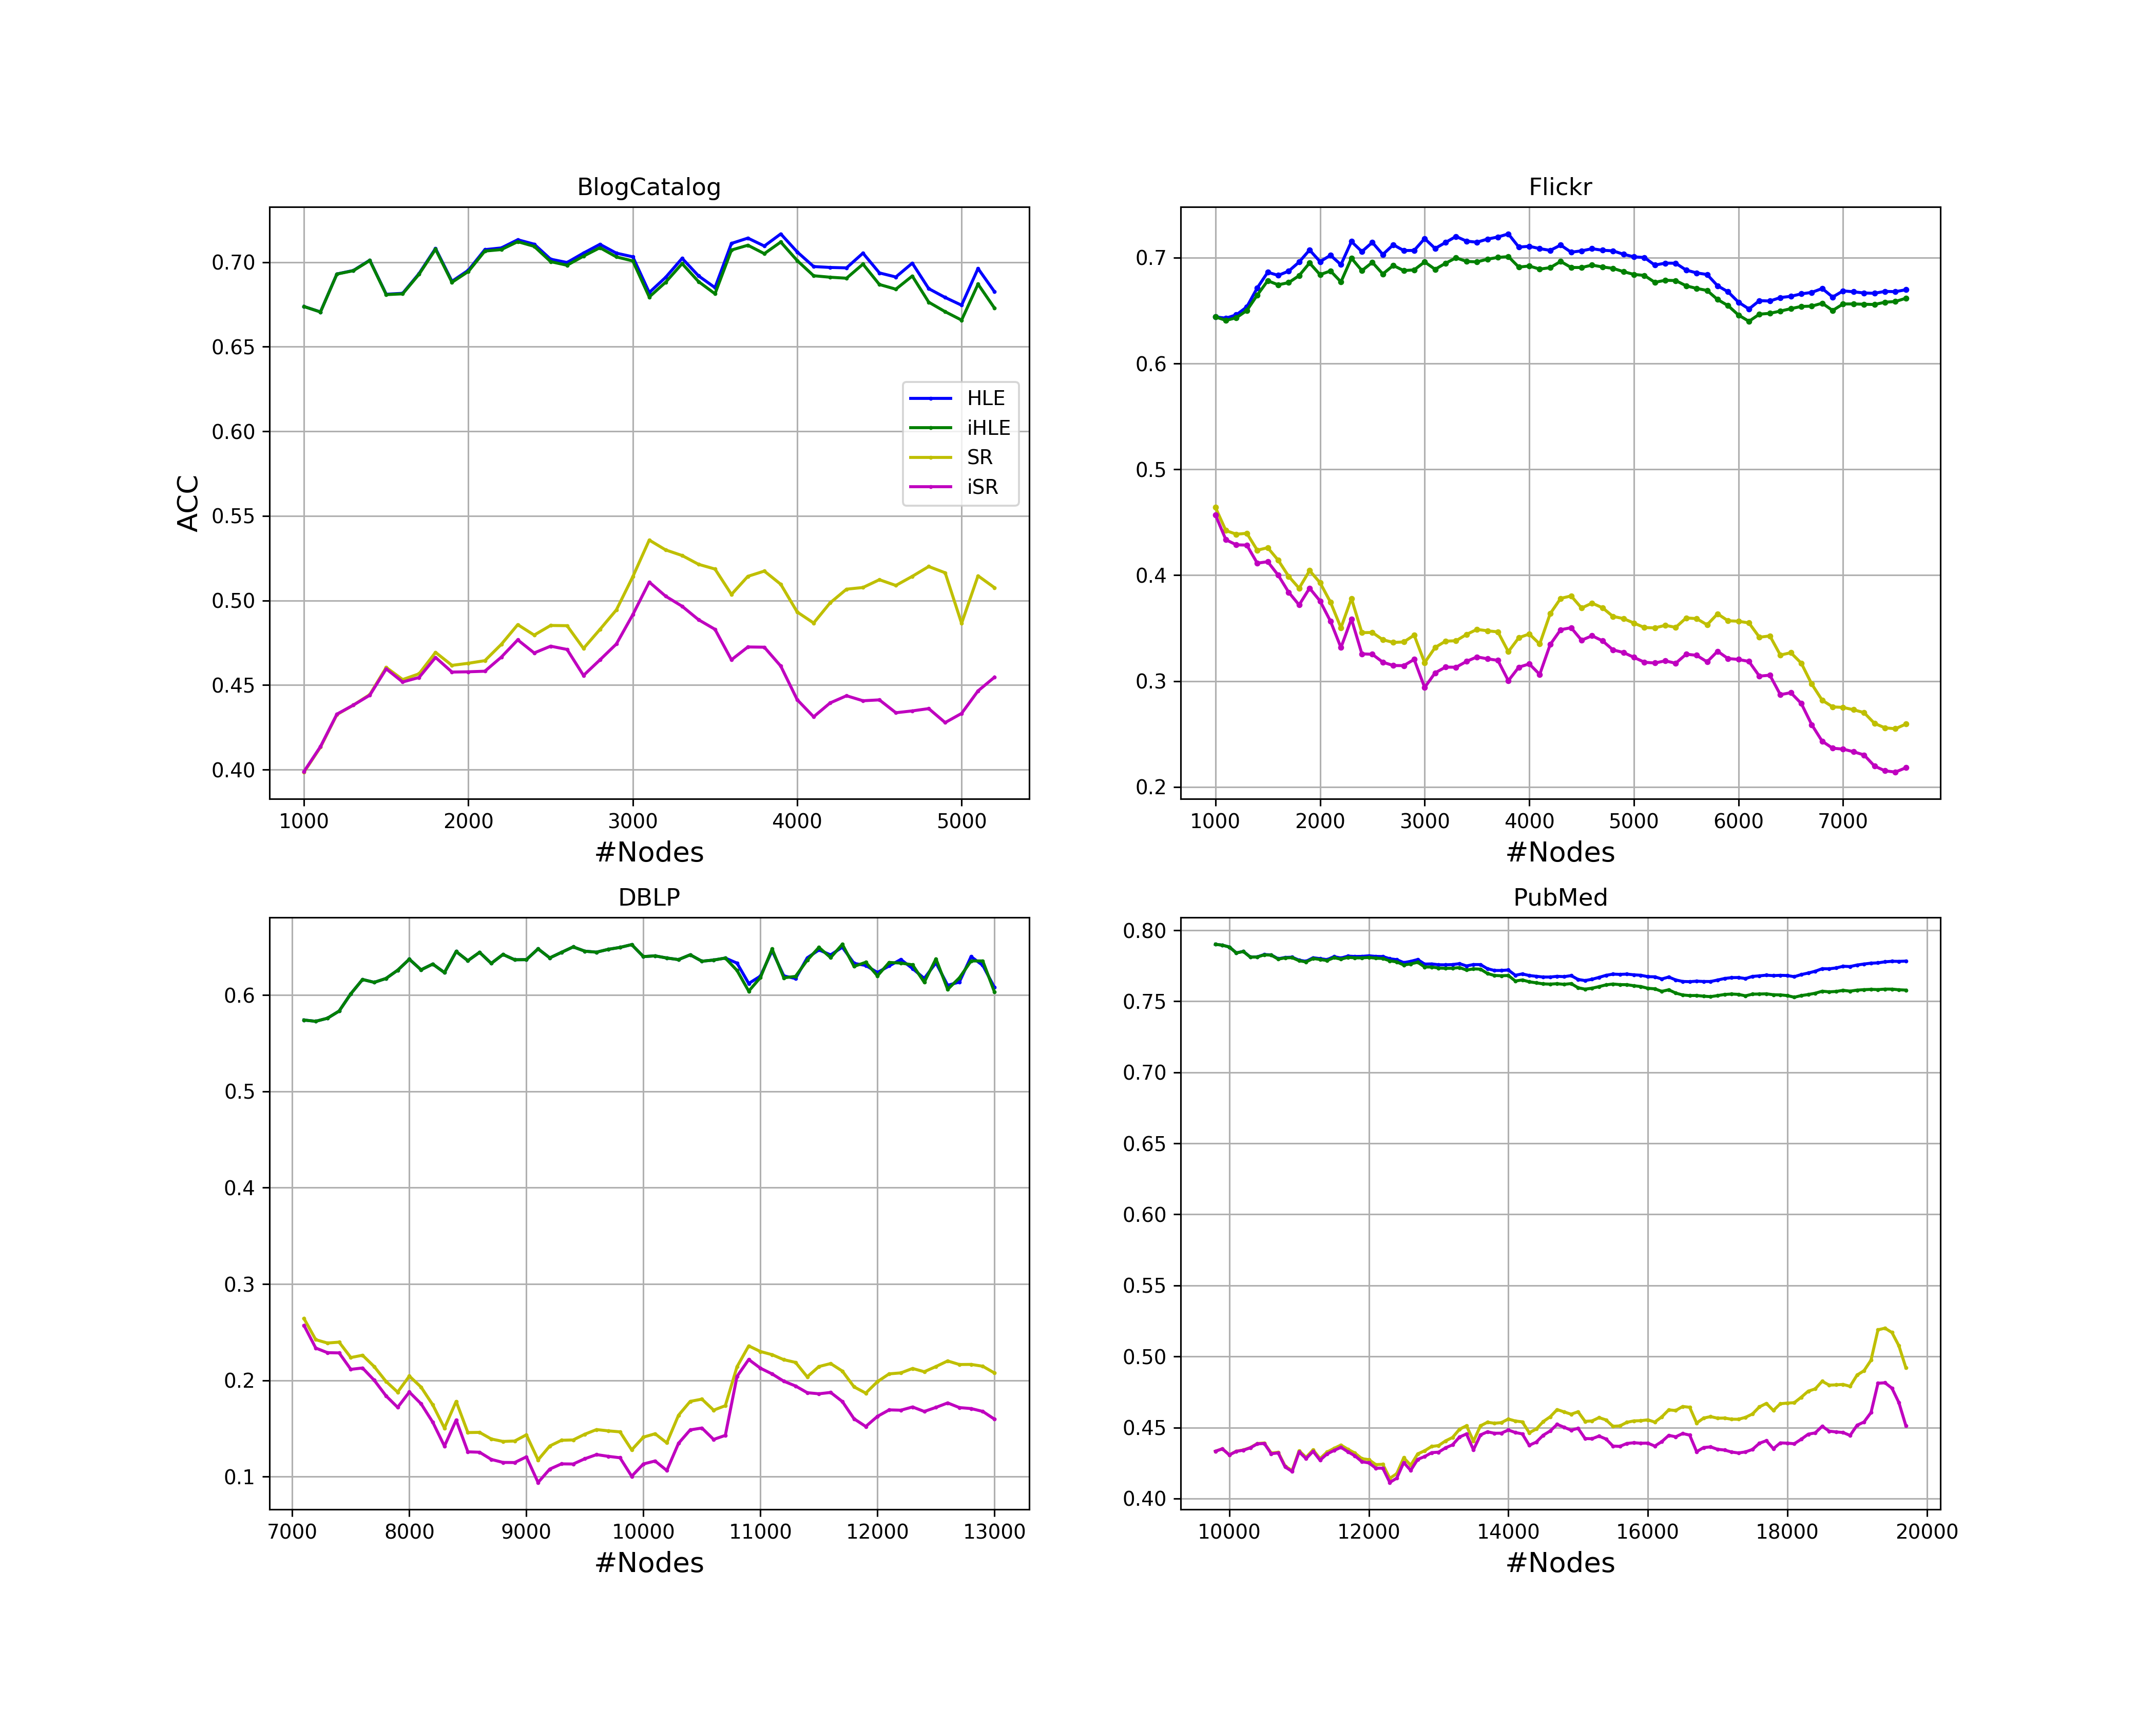
\includegraphics[width=6.5in]{figures/off_vs_on}
	\caption{增量算法与离线算法节点分类任务对比}
	\label{fig:off_vs_on}
\end{figure}

另外,增量算法和离线算法在数据集上的累积误差,定义为在增量学习最后一个时间步时的离线模型和增量模型在节点分类任务上的分类准确率之差。在这里考虑iHLE算法中影响累积误差的因素,其中矩阵变化量$\Delta\textbf{W}$的特征分解维数$m$对累积误差的影响为增量算法的独立参数。通过在PubMed和DBLP数据集上进行实验,对比不同参数情况下累积误差的情况,实验结果如图\ref{fig:parameter_analysis},可以看出特征分解维数$m$和表征向量维数$k$的比值对累积误差的影响较大,随着$m$的增加,累积误差会逐渐减小,在$\frac{m}{k}\approx0.6$时接近最优累积误差,同时可以保证较好的运行效率。

\subsection{运行效率}
为了衡量增量算法的运行效果,本文实验对比了适用属性网络的不同算法包括CCA,ASNE,HLE+SR以及iHLE+SR四种算法在不同数据集上运行的累积时间对比,为控制增量模型对比时间,将四个数据集都分成20个时间步,同一数据集每个时间步之间新增节点数相同,结果如图\ref{fig:runtime}所示。其中横轴为时间步,纵轴为累积运行时间,在BlogCatalog和Flickr数据集上总运行时间较少,增量学习算法的提升效果也不明显,在数据量偏大的DBLP和PubMed数据集中,累积运行时间采用对数坐标,增量学习算法的运行时间明显低于其他算法。
\begin{figure}
	\centering
	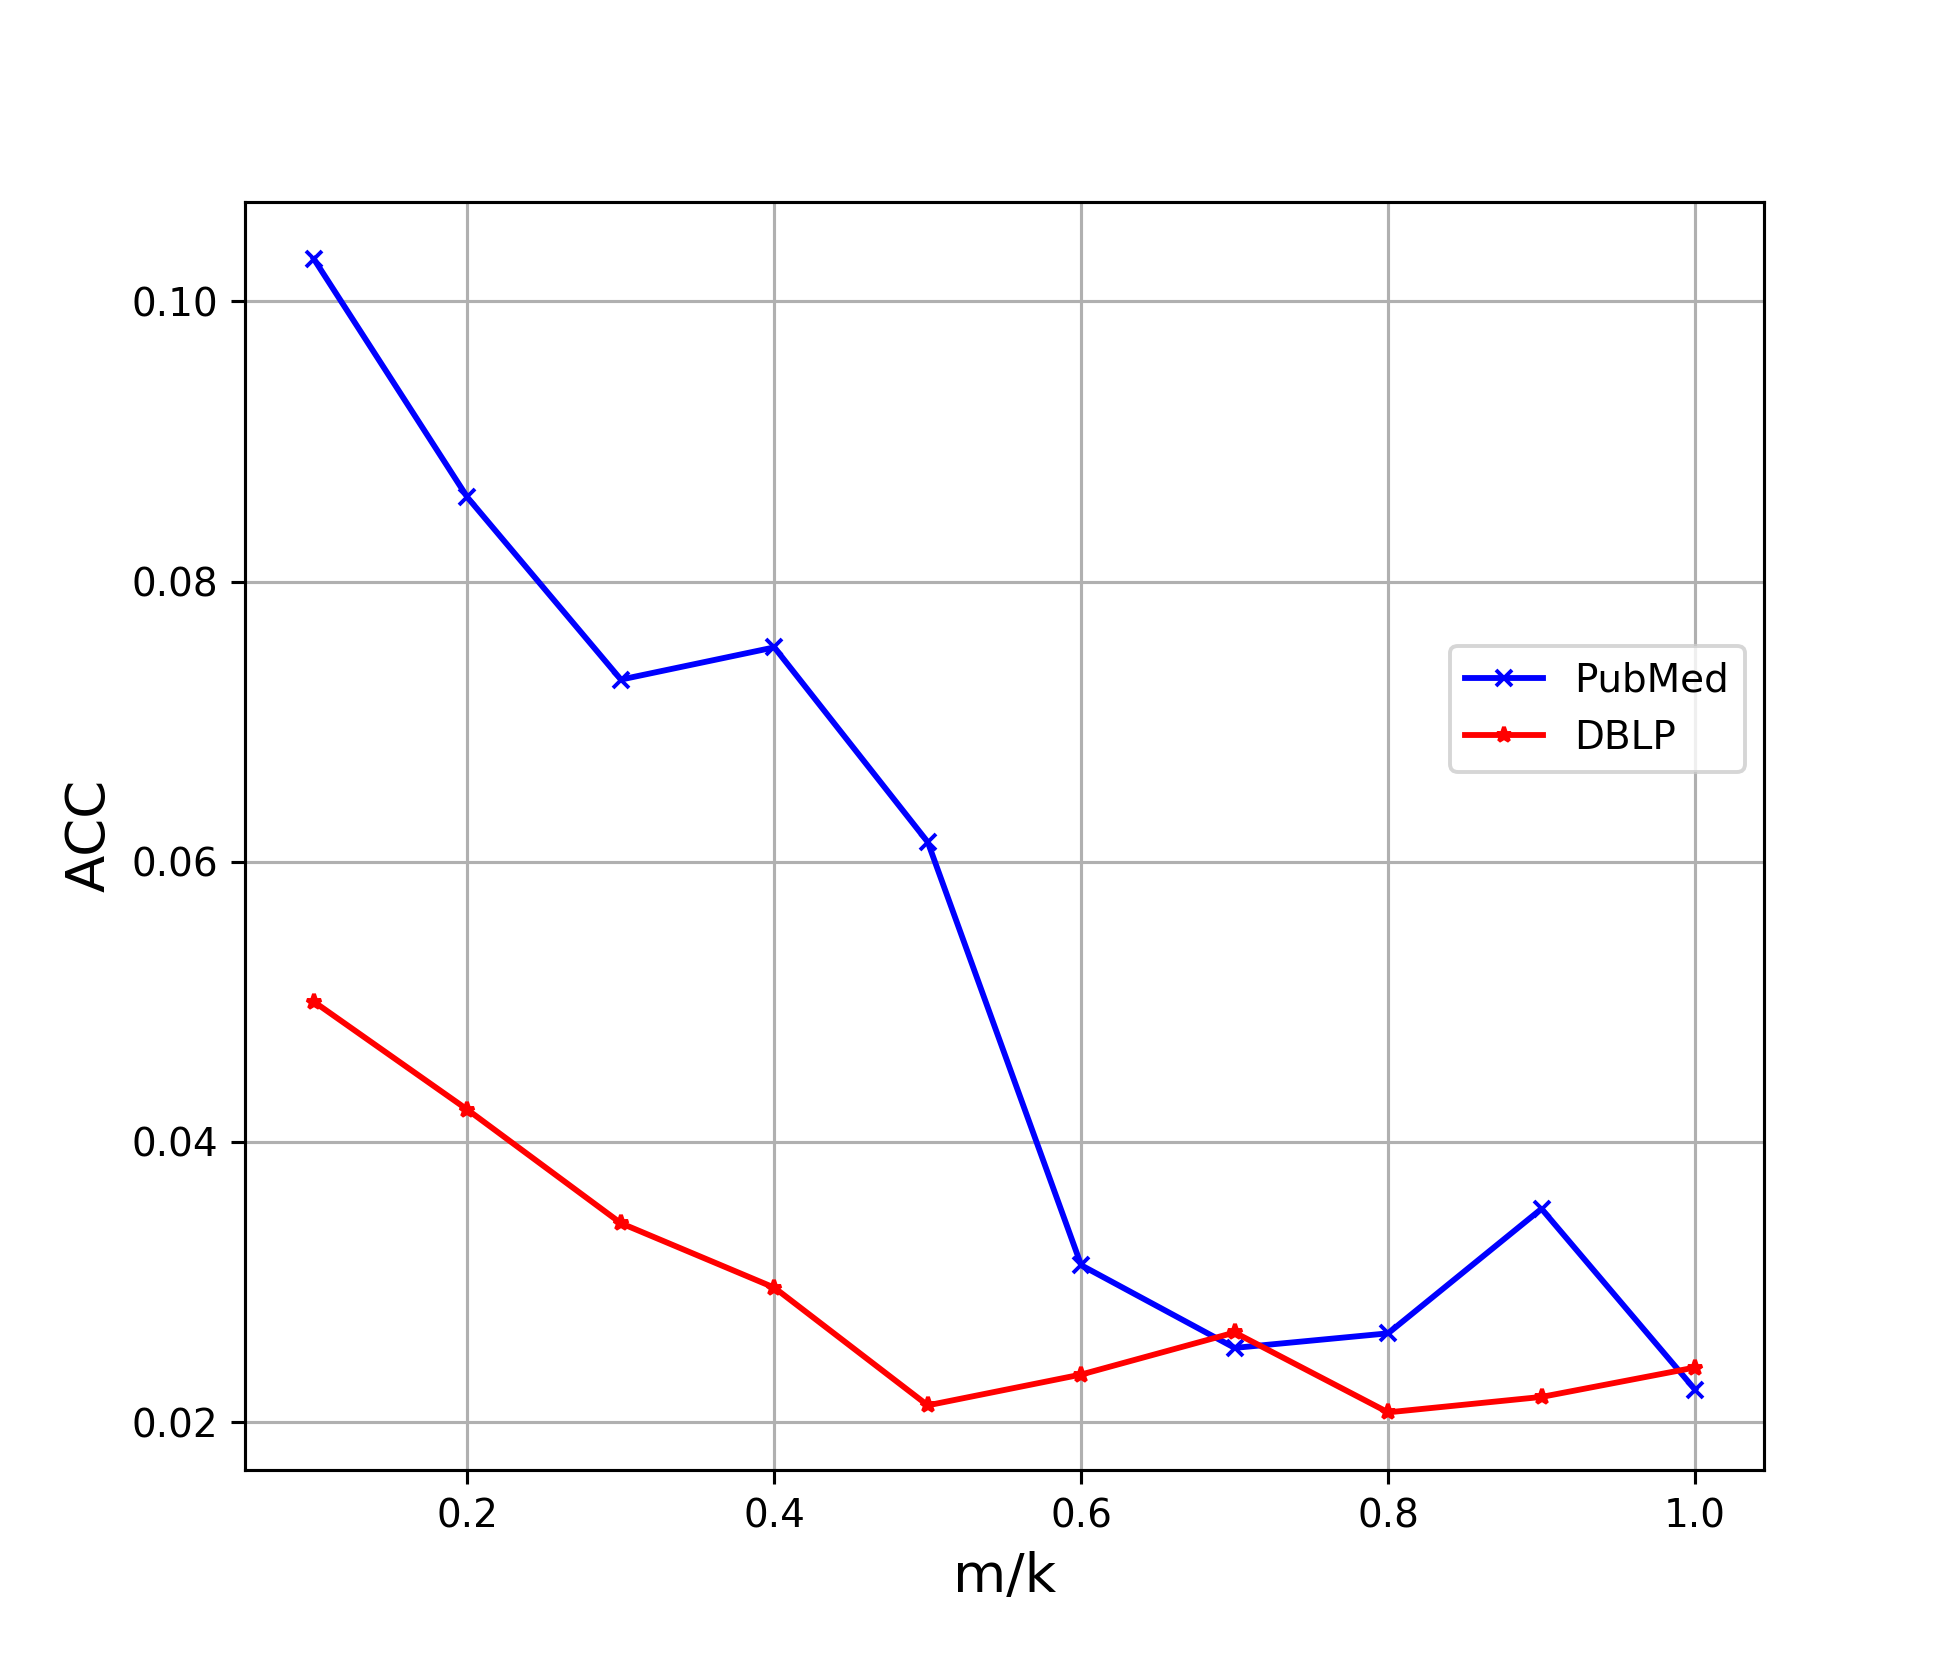
\includegraphics[width=3in]{figures/parameter_analysis}
	\caption{增量矩阵特征分解维度m对节点分类任务的影响}
	\label{fig:parameter_analysis}
\end{figure}

\begin{figure}
	\centering
	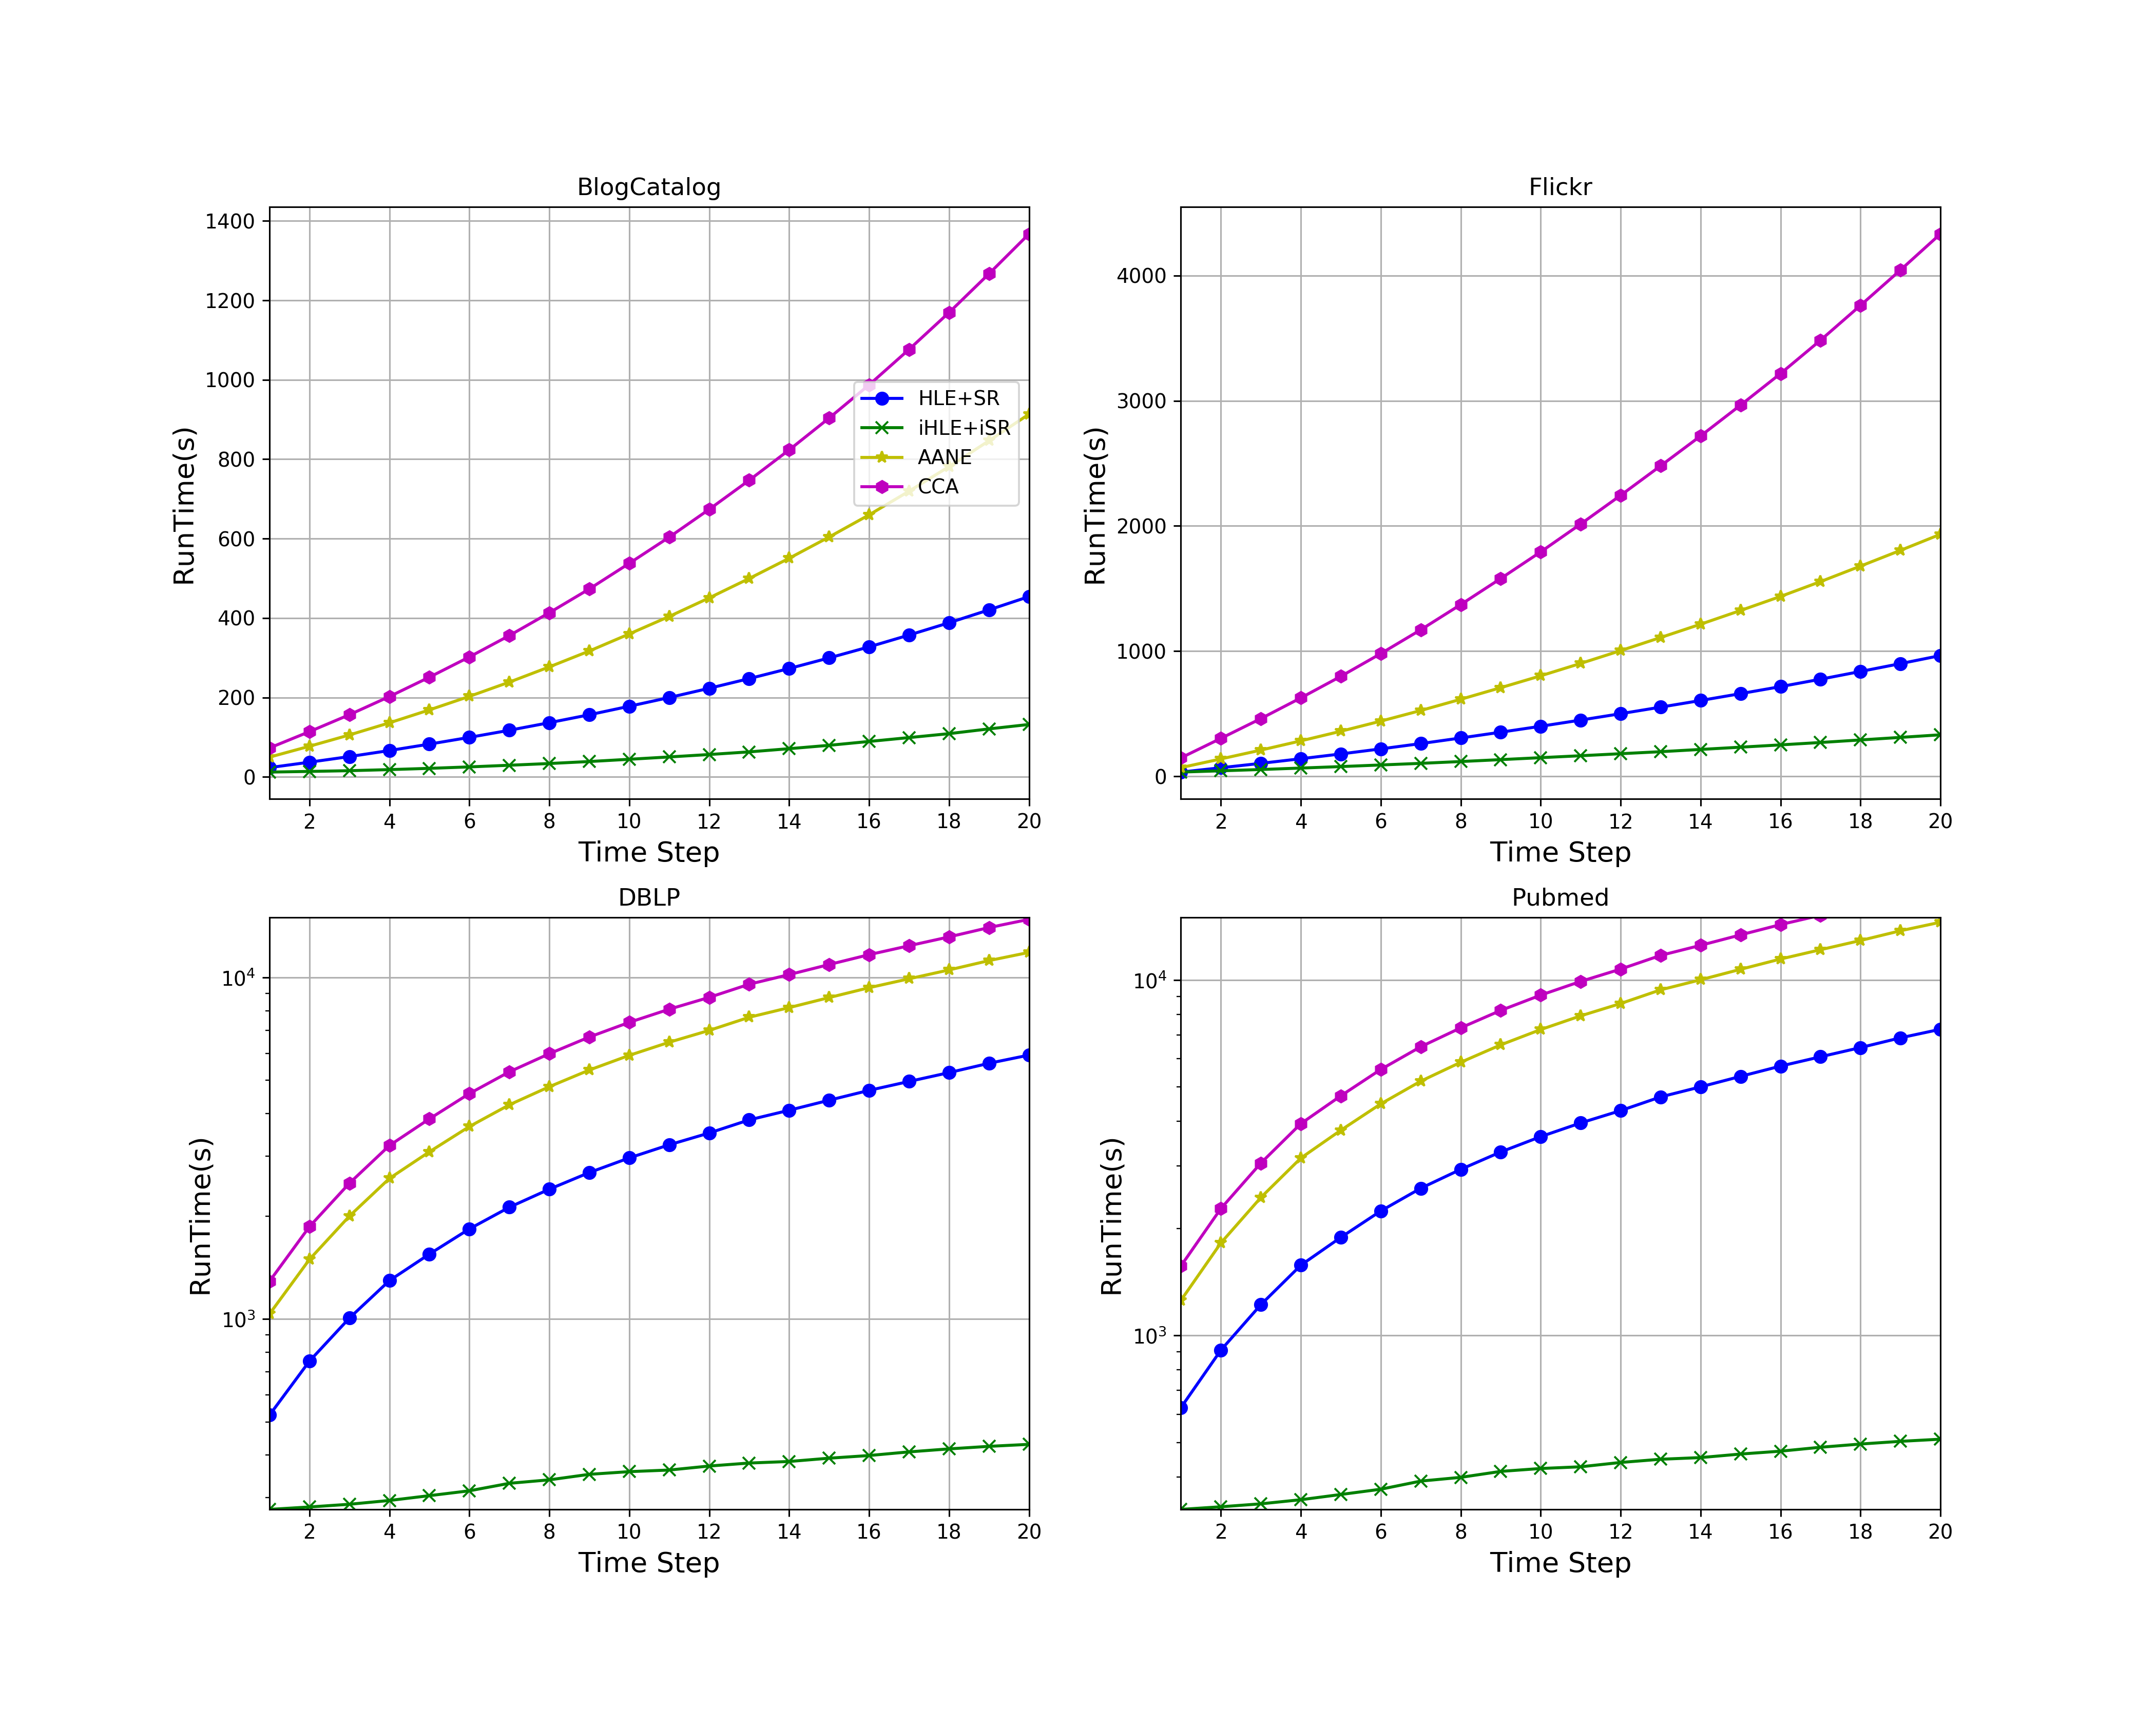
\includegraphics[width=6.5in]{figures/runtime}
	\caption{不同数据集上不同算法的累积运行时间}
	\label{fig:runtime}
\end{figure}

对于增量模型而言,考虑图表征向量维数对运行效率的影响,在不同数据集上进行10次增量过程,对比增量模型和离线模型的平均运行时间,得到在不同表征维数下,增量模型的提速效果,结果如图\ref{fig:dimension_speedup}所示。
\begin{figure}
	\centering
	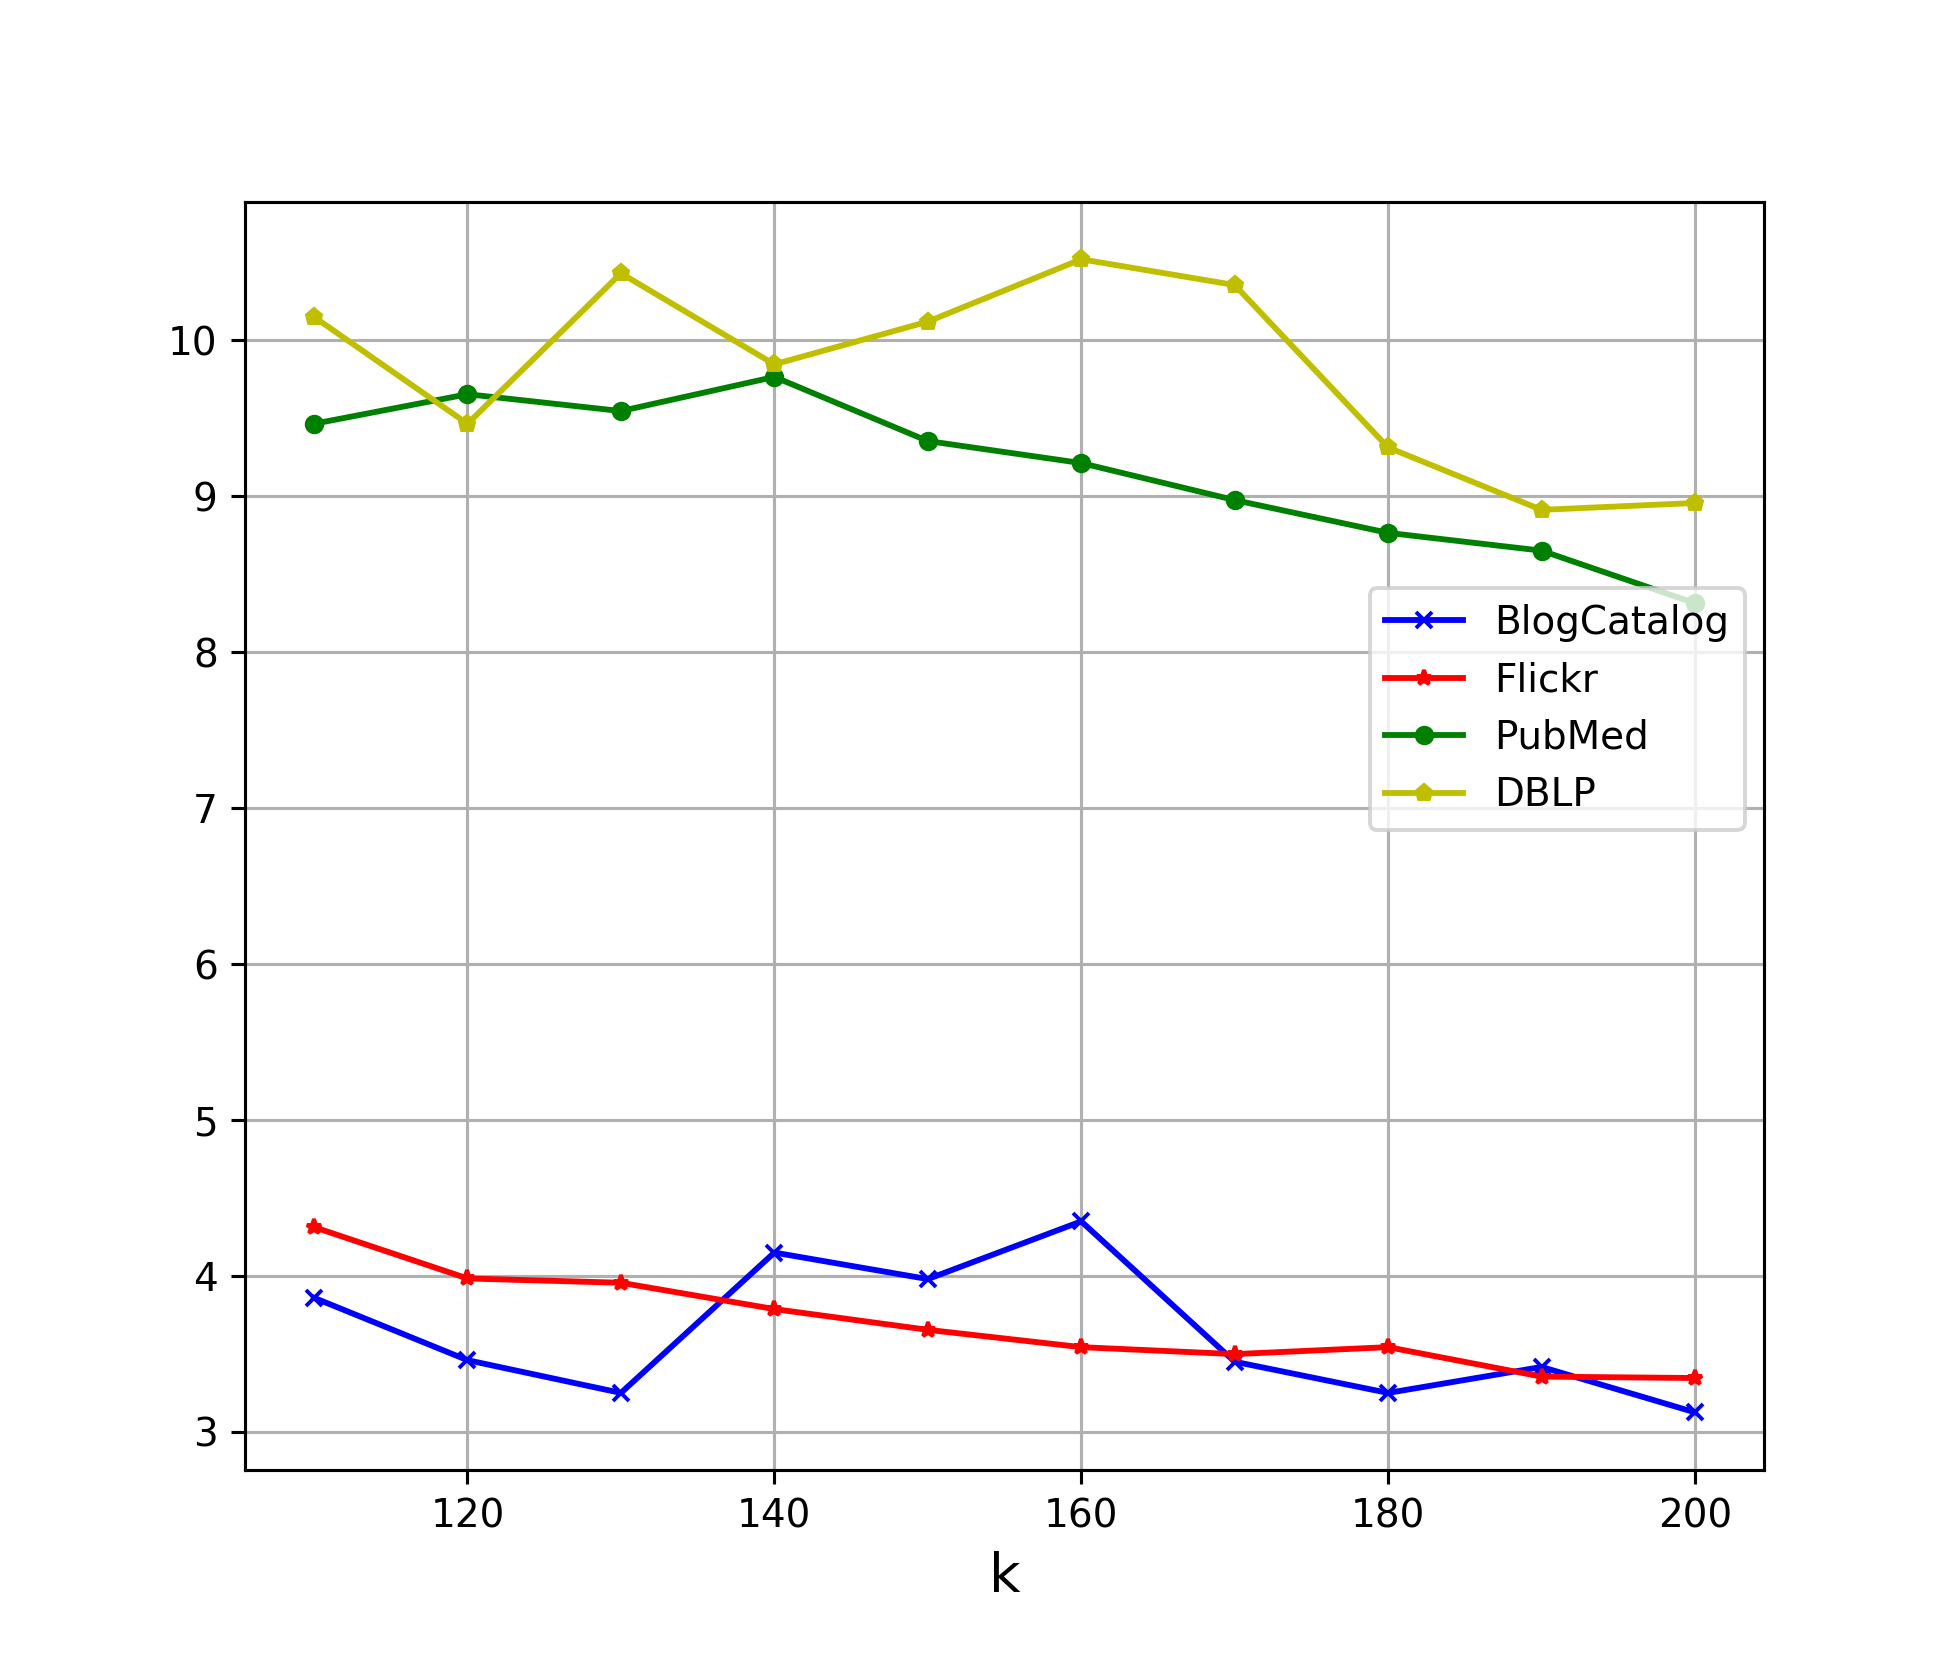
\includegraphics[width=3in]{figures/demension_speedup}
	\caption{增量矩阵特征分解维度m对节}
	\label{fig:dimension_speedup}
\end{figure}

图\ref{fig:dimension_speedup}中纵轴为提速倍数,横轴为图表征向量维数k。其中在模型数据集较小的BlogCatalog和Flickr上,增量模型的提速效果并不明显,约为3-5倍;在数据量较大的DBLP和PubMed上的提速效果较为明显,约为8-10倍。

%%%%%%%%%%%%%%%%%%%%%%%%%%%%%%%%%%%%%%%
%----------------------------------------     本章小结     ---------------------------------------%
%%%%%%%%%%%%%%%%%%%%%%%%%%%%%%%%%%%%%%%
\section{本章小结}
本章中从两个方面来对算法效果进行衡量:准确性评估和运行效率评估,其中准确性评估从节点分类和链路预测两个机器学习任务来进行评估。在节点分类任务中HLE算法和SR1算法明显优于其他对比算法;在链路预测任务中,基于结构的HLE算法仍保持比较好的分类效果,基于节点属性的SR1算法效果不够理想。对于增量模型的准确性评估,主要采用了与相应的离线模型在节点分类任务中的预测准确率差异进行评估,iHLE算法和iSR算法都表现出很好的稳定性,同时对影响累积误差的参数进行了实验分析。

在运行效率评估方面,通过对比增量模型和离线模型在对应时间步上的累积运行时间对算法的运行效率进行评估,iHLE+iSR算法效果表现出很好的运行效率,在小数据集BlogCatalog和Flickr上表现出3-5倍的提速效果,在偏大的数据集PubMed和DBLP上表现出8-10倍的提速效果,同时实验对影响运行效率的因素进行了实验分析。